%================================================================
% SLO
%----------------------------------------------------------------
% datoteka: 	thesis_template.tex
%
% opis: 		predloga za pisanje diplomskega dela v formatu LaTeX na
% 				Univerza v Ljubljani, Fakulteti za računalništvo in informatiko
%
% pripravili: 	Matej Kristan, Zoran Bosnić, Andrej Čopar,
%			  	po začetni predlogi Gašperja Fijavža
%
% popravil: 	Domen Rački, Jaka Cikač, Matej Kristan
%
% verzija: 		30. september 2016 (dodan razširjeni povzetek)
%================================================================


%================================================================
% SLO: definiraj strukturo dokumenta
% ENG: define file structure
%================================================================
\documentclass[a4paper, 12pt]{book}
 

%================================================================
% SLO: Odkomentiraj "\SLOtrue " za izbiro slovenskega jezika
% ENG: Uncomment "\SLOfalse" to chose English languagge
%================================================================
\newif\ifSLO
\newif\ifTRACKEXIST
\newif\ifTRACKCS
\newif\ifPROGRAMMM

% ---------------------------------------------------------------------------------------
% IMPORTANT: Adjust the thesis language, your study program and course within this block
% ---------------------------------------------------------------------------------------
% switch language
%\SLOtrue % Enables Slovenian language
\SLOfalse  % Enables English language

% switch programs: Computer science and Multimedia. Set to false if the program is in Multimedia
\PROGRAMMMfalse
%\PROGRAMMMtrue

% switch on if your program is divided into tracks CS and DS, otherwise leave it false
% CAUTION: if you were first enrolled into your program before school year 2019/2020, your program is not divided into tracks. In any case, be absolutely sure you select the correct variant. IF IN DOUBT, always contact the student office to advise you.
%
 \TRACKEXISTfalse
%\TRACKEXISTtrue

% default course name is "Computer science" if your course name is "Data science", set the following switch to false
\TRACKCStrue % uncomment if the thesis is from course "Information science"
%\TRACKCSfalse % uncomment if the thesis is from course "Data Science"
% -------------------------------------------------------------------------------------------
% End of language, program and course adjustment
% -------------------------------------------------------------------------------------------


%================================================================
% SLO: vključi oblikovanje in pakete
% ENG: include design and packages
%================================================================
%----------------------------------------------------------------
% SLO: LaTeX paketi
% ENG: LateX packages
%----------------------------------------------------------------
% SLO: omogoča uporabo slovenskih (latinskih) črk kodiranih v formatu UTF-8
% ENG: enables the use of slovene (latin) caracters encoded in the UFT-8 format
\usepackage[utf8x]{inputenc}
%\inputencoding{utf8}
% SLO: naloži, med drugim, slovenske delilne vzorce
% ENG: loads, among others, slovene dividing patterns
\usepackage[slovene,english]{babel}
% SLO: poskrbi za postavitev strani
% ENG: takes care of the page layout
\usepackage{fancyhdr}
% SLO: za vlaganje slik različnih formatov
% ENG: for loading figures of different formats
\usepackage{graphicx}
\usepackage{caption}
\captionsetup[figure]{labelfont=bf} % SLO: napis "Slika #" v krepkem tisku
									% ENG: wirte "Figure #" caption in bold
\captionsetup[table]{labelfont=bf} % SLO: napis "Tabela #" v krepkem tisku
								   % ENG: wirte "Table #" caption in bold
% SLO: za pisanje psevdokode
% ENG: for writing pseudocode
\usepackage{algorithm}
\usepackage{algorithmic}
\floatname{algorithm}{\footnotesize Algorithm} % SLO: napis "Algoritem #" v krepkem tisku
											   % ENG: write "Algorithm #" caption in bold
% SLO: poveže reference slik/tabel in slike/tabele znotraj dokumenta
% ENG: links image/table references with the images/tables within the document
\usepackage[pdfa]{hyperref}
% SLO: pri kliku na referenco slike/tabele se postavi na vrh slike/tabele
% ENG: when clicking the image/table reference, position the focus on top of the image/table
\usepackage[all]{hypcap}
% SLO: omogoča, med drugim, definicjo in uporebo barve
% ENG: enables, among others, the definition and use of colors
\usepackage{xcolor}
%----------------------------------------------------------------
% SLO: dodatni paketi
% ENG: additional packages
%----------------------------------------------------------------
% SLO: omogoča večjo manipulacijo nad tabelami
% ENG: allows for greater manipulation of tables
\usepackage{booktabs}
% SLO: naloži dodatne simbole
% ENG: loads additional symbols
\usepackage{amssymb}
% SLO: omogoča, med drugim, sklicevanje na formule z eqref
% ENG: enables, among others, equation referencing with eqref
\usepackage{amsmath}
% SLO: omogoča komentiranje večjega dela teksta
% ENG: enables the commenting of larger text parts
\usepackage{verbatim}
% SLO: omogoča rotacijo PDF strani v ležeč položaj
% ENG: enables the rotation of a PDF page to landscape
\usepackage{pdflscape}
% SLO: omogoča barvanje vrstic in stolpcev tabel
% ENG: enables coloring of table rows and columns
\usepackage{colortbl}
\usepackage{url}



%================================================================
% SLO: nastavitve dokumenta
% ENG: document properties
%================================================================
% SLO: prilagoditev robov za tisk
% ENG: margin adjustments for printing
\addtolength{\marginparwidth}{-20pt}
\addtolength{\oddsidemargin}{40pt}
\addtolength{\evensidemargin}{-40pt}
% SLO: razmik med vrsticami
% ENG: line spacing
\renewcommand{\baselinestretch}{1.3}
% SLO: postavitev strani
% ENG: page layout
\renewcommand{\chaptermark}[1]{\markboth{\MakeUppercase{\thechapter.\ #1}}{}}
\renewcommand{\sectionmark}[1]{\markright{\MakeUppercase{\thesection.\ #1}}}
\renewcommand{\headrulewidth}{0.5pt} % Header rule
\renewcommand{\footrulewidth}{0pt} % Footer rule
%
\fancypagestyle{frontmatter}{%
	\fancyhf{} % Clear all headers and footers first
	\fancyhead[LE, RO]{\sl \thepage}
	%\fancyhead[LO]{\sl \rightmark}
	%\fancyhead[RE]{\sl \leftmark}
}
\fancypagestyle{mainmatter}{%
  	\fancyhf{} % Clear all headers and footers first
	\fancyhead[LE,RO]{\sl \thepage}
	\fancyhead[LO]{\sl \rightmark}
	\fancyhead[RE]{\sl \leftmark}
}
% SLO: font za ime avtorja
% ENG: font for author name
\newcommand{\authorfont}{\Large}
% SLO: font za naslov diplomskega dela
% ENG: font for thesis title
\newcommand{\titlefont}{\LARGE\bf}
% SLO: globina kazala
% ENG: content depth
\setcounter{tocdepth}{1}
% SLO: definiraj ukaz za prazno stran
% ENG: define the command for empty page
\newcommand{\clearemptydoublepage}{\newpage{\pagestyle{empty}\cleardoublepage}}

% course title
\newcommand{\trackname}{!undefined!}

\newcommand{\BibTeX}{{\sc Bib}\TeX}




%----------------------------------------------------------------
% |||||||||||||||||||||| USTREZNO POPRAVI |||||||||||||||||||||||
% |||||||||||||||||||||| EDIT ACCORDINGLY |||||||||||||||||||||||
%----------------------------------------------------------------
\newcommand{\ttitle}{Primerjava uspešnosti odprtokodnih in komercialnih orodij za luščenje podatkov}
\newcommand{\ttitleEn}{Performance comparison of open source and commercial information extraction tools}
\newcommand{\tsubject}{\ttitle}
\newcommand{\tsubjectEn}{\ttitleEn}
\newcommand{\tauthor}{Romana Grilj}
\newcommand{\temail}{romana.grilj@gmai.com}
\newcommand{\myyear}{2023}
\newcommand{\tkeywords}{analiza podatkov, ekstrakcija podatkov, strukturni podatki, spletno rudarjenje}
\newcommand{\tkeywordsEn}{Data analysis, Information Retrieval, structural data, Web Mining}
\newcommand{\mysupervisor}{doc.~dr.\ Slavko Žitnik}
%\newcommand{\mycosupervisor}{akad.~prof.~dr.\ Martin Krpan}
% include formatted front pages

%----------------------------------------------------------------
% SLO: definiraj metapodatke za datoteko thesis_template.tex
% ENG: define metadata for the file thesis_template.tex
%----------------------------------------------------------------
%----------------------------------------------------------------
%	HYPERREF SETUP
% SLO: ustrezno popravi e-mail
% ENG: edit the e-mail accordingly
%----------------------------------------------------------------
\hypersetup{pdftitle={\ttitle}}
\hypersetup{pdfsubject=\ttitleEn}
\hypersetup{pdfauthor={\tauthor, \temail}}
\hypersetup{pdfkeywords=\tkeywordsEn}

%----------------------------------------------------------------
% define medatata
% SLO: ustrezno popravi e-mail
% ENG: edit the e-mail accordingly
%----------------------------------------------------------------
\def\Title{\ttitle}
\def\Author{\tauthor, \temail}
\def\Subject{\ttitleEn}
\def\Keywords{\tkeywordsEn}
\def\Org{Univerza v Ljubljani, Fakulteta za računalništvo in informatiko}

%%%%%%%%%%%%%%%%%%%%%%%%%%%%%%%%%%%%%%%%
% \convertDate converts D:20080419103507+02'00' to 2008-04-19T10:35:07+02:00
%%%%%%%%%%%%%%%%%%%%%%%%%%%%%%%%%%%%%%%%
\def\convertDate{%
    \getYear
}

{\catcode`\D=12
 \gdef\getYear D:#1#2#3#4{\edef\xYear{#1#2#3#4}\getMonth}
}
\def\getMonth#1#2{\edef\xMonth{#1#2}\getDay}
\def\getDay#1#2{\edef\xDay{#1#2}\getHour}
\def\getHour#1#2{\edef\xHour{#1#2}\getMin}
\def\getMin#1#2{\edef\xMin{#1#2}\getSec}
\def\getSec#1#2{\edef\xSec{#1#2}\getTZh}
\def\getTZh +#1#2{\edef\xTZh{#1#2}\getTZm}
\def\getTZm '#1#2'{%
    \edef\xTZm{#1#2}%
    \edef\convDate{\xYear-\xMonth-\xDay T\xHour:\xMin:\xSec+\xTZh:\xTZm}%
}

\expandafter\convertDate\pdfcreationdate


%%%%%%%%%%%%%%%%%%%%%%%%%%%%%%%%%%%%%%%%
% get pdftex version string
%%%%%%%%%%%%%%%%%%%%%%%%%%%%%%%%%%%%%%%%
\newcount\countA
\countA=\pdftexversion
\advance \countA by -100
\def\pdftexVersionStr{pdfTeX-1.\the\countA.\pdftexrevision}

%%%%%%%%%%%%%%%%%%%%%%%%%%%%%%%%%%%%%%%%
% XMP data
%%%%%%%%%%%%%%%%%%%%%%%%%%%%%%%%%%%%%%%%
\usepackage{xmpincl}
\includexmp{pdfa-1b}

%%%%%%%%%%%%%%%%%%%%%%%%%%%%%%%%%%%%%%%%
% pdfInfo
%%%%%%%%%%%%%%%%%%%%%%%%%%%%%%%%%%%%%%%%
\pdfinfo{%
    /Title    (\ttitle)
    /Author   (\tauthor, \temail)
    /Subject  (\ttitleEn)
    /Keywords (\tkeywordsEn)
    /ModDate  (\pdfcreationdate)
    /Trapped  /False
}

%================================================================
% SLO: razno
% ENG: other
%================================================================
% SLO: nastavitev sklicevanj
% ENG: hyper referencing setup
\definecolor{black}{rgb}{0,0,0}
\hypersetup{
	colorlinks = true,
	linkcolor = black,
	citecolor = black,
	urlcolor = black
}

%----------------------------------------------------------------
% SLO: dodaj poti do datotek s slikami
% ENG: add paths to files containing figures
%----------------------------------------------------------------
\graphicspath{
	{figures/}
	{tables/}
}
%----------------------------------------------------------------
% SLO: moji paketi
% ENG: my packages
%----------------------------------------------------------------
% ...
%----------------------------------------------------------------
% SLO: moji konstrukti
% ENG: my constructs
%----------------------------------------------------------------
\newtheorem{izrek}{Izrek}[chapter]
\newtheorem{trditev}{Trditev}[izrek]
\newenvironment{dokaz}{\emph{Dokaz.}\ }{\hspace{\fill}{$\Box$}}

\newcommand{\CcImageCc}[1]{%
	
\includegraphics[scale=#1]{cc-licenca/cc_cc_30.pdf}%
}
\newcommand{\CcImageBy}[1]{%
	
\includegraphics[scale=#1]{cc-licenca/cc_by_30.pdf}%
}
\newcommand{\CcImageSa}[1]{%
	
\includegraphics[scale=#1]{cc-licenca/cc_sa_30.pdf}%
}


%================================================================
% SLO: začetne strani magistrskega dela
% ENG: fist pages of the master's thesis
%================================================================
\begin{document}
% SLO: prepreči težave s številkami strani v kazalu
% ENG: prevents problems with the page numbers in the contents page
\renewcommand{\thepage}{}

%----------------------------------------------------------------
% Language-dependent formatting
%----------------------------------------------------------------
\ifSLO
    % SLO: definiraj slovensko besedo za kazalo
    \renewcommand{\contentsname}{Kazalo}

    % SLO: naslovnica
    % select the course title if it exist
\ifTRACKEXIST
    \ifTRACKCS
        \renewcommand{\trackname}{Računalništvo in Informatika}
    \else
        \renewcommand{\trackname}{Podatkovne Vede}
    \fi
\fi

\ifPROGRAMMM
    \thispagestyle{empty}
    \begin{center}
        {\large\sc Univerza v Ljubljani\\Fakulteta za računalništvo in informatiko\\
            Fakulteta za elektrotehniko}
    	   \vskip 10em
    	   {\authorfont \tauthor \par}
    	   {\titlefont \ttitle \par}
        {\vskip 2em \textsc{MAGISTRSKO DELO\\[2mm]
        MAGISTRSKI ŠTUDIJSKI PROGRAM DRUGE STOPNJE\\MULTIMEDIJA
        }\par}
        \vfill\null
        {\large \textsc{Mentor}: \mysupervisor \par}
   %	    {\large \textsc{Somentor}: \mycosupervisor \par}
        {\vskip 2em \large Ljubljana, \myyear \par}
   \end{center}
\else
    \thispagestyle{empty}
	\begin{center}
            {\large\sc Univerza v Ljubljani\\Fakulteta za računalništvo in informatiko}
    	   \vskip 10em
    	   {\authorfont \tauthor \par}
    	   {\titlefont \ttitle \par}
        {\vskip 2em \textsc{MAGISTRSKO DELO\\[2mm]
        MAGISTRSKI ŠTUDIJSKI PROGRAM DRUGE STOPNJE\\RAČUNALNIŠTVO IN INFORMATIKA
        \ifTRACKEXIST
            \\Smer: \trackname
        \fi
        }\par}
        \vfill\null
        {\large \textsc{Mentor}: \mysupervisor \par}
   %	    {\large \textsc{Somentor}: \mycosupervisor \par}
        {\vskip 2em \large Ljubljana, \myyear \par}
   \end{center}
\fi  \clearemptydoublepage
    % SLO: avtorske pravice
    \thispagestyle{empty}
\vspace*{\fill}
{\noindent\footnotesize


\vspace*{5cm}
{\small \noindent
To delo je ponujeno pod licenco \textit{Creative Commons Priznanje avtorstva-Deljenje pod enakimi pogoji 2.5 Slovenija} (ali novej\v so razli\v cico).
To pomeni, da se tako besedilo, slike, grafi in druge sestavine dela kot tudi rezultati diplomskega dela lahko prosto distribuirajo,
reproducirajo, uporabljajo, priobčujejo javnosti in predelujejo, pod pogojem, da se jasno in vidno navede avtorja in naslov tega
dela in da se v primeru spremembe, preoblikovanja ali uporabe tega dela v svojem delu, lahko distribuira predelava le pod
licenco, ki je enaka tej.
Podrobnosti licence so dostopne na spletni strani \href{http://creativecommons.si}{creativecommons.si} ali na Inštitutu za
intelektualno lastnino, Streliška 1, 1000 Ljubljana.

\begin{center}% 0.66 / 0.89 = 0.741573033707865
\CcImageCc{0.741573033707865}\hspace*{1ex}\CcImageBy{1}\hspace*{1ex}\CcImageSa{1}%
\end{center}
}

\vspace*{1.5cm}
{\small \noindent
Izvorna koda diplomskega dela, njeni rezultati in v ta namen razvita programska oprema je ponujena pod licenco GNU General Public License,
različica 3 (ali novejša). To pomeni, da se lahko prosto distribuira in/ali predeluje pod njenimi pogoji.
Podrobnosti licence so dostopne na spletni strani \url{http://www.gnu.org/licenses/}.
}


}
\begin{center}
{\footnotesize{\sc \copyright \myyear\ \tauthor}}
\end{center}  \clearemptydoublepage
    % SLO: izjava o avtorstvu (ni več del vezane izdaje, ločena oddaja)
    % SLO: zahvala
    \thispagestyle{empty}

\begin{center}
{\Large \textbf{\sc Zahvala}}
\end{center}
\vspace{0.5cm}

{\it\noindent
Na tem mestu zapišite, komu se zahvaljujete za izdelavo magistrske naloge. V zahvali se poleg mentorja spodobi omeniti vse, ki so s svojo pomočjo prispevali k nastanku vašega izdelka.

\vspace{0.5cm} \hfill \tauthor, \myyear
} \clearemptydoublepage
    % SLO: posvetilo
    \thispagestyle{empty}\mbox{}{\vskip0.20\textheight}\mbox{}\hfill\begin{minipage}{0.55\textwidth}%

Vsem rožicam tega sveta.\\\\
\textit{''The only reason for time is so that everything doesn't happen at once.''}
\flushright --- Albert Einstein
\normalfont\end{minipage} \clearemptydoublepage
\else

    % ENG: title page ENG
    % select the course title if it exist
\ifTRACKEXIST
    \ifTRACKCS
        \renewcommand{\trackname}{Computer and Information Science}
    \else
        \renewcommand{\trackname}{Data Science}
    \fi
\fi

\ifPROGRAMMM
    \thispagestyle{empty}
	\begin{center}
        {\large\sc University of Ljubljana\\Faculty of Computer and Information Science\\
        Faculty of Electrical Engineering}
    	\vskip 10em
    	{\authorfont \tauthor \par}
    	{\titlefont \ttitleEn \par}
        {\vskip 2em \textsc{MASTER'S THESIS\\[2mm]
        THE 2nd CYCLE MASTER'S STUDY PROGRAMME\\MULTIMEDIA
        }\par}
        \vfill\null
        {\large \textsc{Supervisor}: \mysupervisor \par}
   	 %   {\large \textsc{Co-supervisor}:  \mycosupervisor \par}
        {\vskip 2em \large Ljubljana, \myyear \par}
   \end{center}
\else
    \thispagestyle{empty}
	\begin{center}
        {\large\sc University of Ljubljana\\Faculty of Computer and Information Science}
    	\vskip 10em
    	{\authorfont \tauthor \par}
    	{\titlefont \ttitleEn \par}
        {\vskip 2em \textsc{MASTER'S THESIS\\[2mm]
        THE 2nd CYCLE MASTER'S STUDY PROGRAMME\\COMPUTER AND INFORMATION SCIENCE
        \ifTRACKEXIST
            \\Track: \trackname
        \fi
        }\par}
        \vfill\null
        {\large \textsc{Supervisor}: \mysupervisor \par}
   	%    {\large \textsc{Co-supervisor}:  \mycosupervisor \par}
        {\vskip 2em \large Ljubljana, \myyear \par}
    \end{center}
\fi  \clearemptydoublepage
    % ENG: title page SLO
    % select the course title if it exist
\ifTRACKEXIST
    \ifTRACKCS
        \renewcommand{\trackname}{Računalništvo in Informatika}
    \else
        \renewcommand{\trackname}{Podatkovne Vede}
    \fi
\fi

\ifPROGRAMMM
    \thispagestyle{empty}
    \begin{center}
        {\large\sc Univerza v Ljubljani\\Fakulteta za računalništvo in informatiko\\
            Fakulteta za elektrotehniko}
    	   \vskip 10em
    	   {\authorfont \tauthor \par}
    	   {\titlefont \ttitle \par}
        {\vskip 2em \textsc{MAGISTRSKO DELO\\[2mm]
        MAGISTRSKI ŠTUDIJSKI PROGRAM DRUGE STOPNJE\\MULTIMEDIJA
        }\par}
        \vfill\null
        {\large \textsc{Mentor}: \mysupervisor \par}
   %	    {\large \textsc{Somentor}: \mycosupervisor \par}
        {\vskip 2em \large Ljubljana, \myyear \par}
   \end{center}
\else
    \thispagestyle{empty}
	\begin{center}
            {\large\sc Univerza v Ljubljani\\Fakulteta za računalništvo in informatiko}
    	   \vskip 10em
    	   {\authorfont \tauthor \par}
    	   {\titlefont \ttitle \par}
        {\vskip 2em \textsc{MAGISTRSKO DELO\\[2mm]
        MAGISTRSKI ŠTUDIJSKI PROGRAM DRUGE STOPNJE\\RAČUNALNIŠTVO IN INFORMATIKA
        \ifTRACKEXIST
            \\Smer: \trackname
        \fi
        }\par}
        \vfill\null
        {\large \textsc{Mentor}: \mysupervisor \par}
   %	    {\large \textsc{Somentor}: \mycosupervisor \par}
        {\vskip 2em \large Ljubljana, \myyear \par}
   \end{center}
\fi  \clearemptydoublepage
    % ENG: copyright
    \thispagestyle{empty}
\vspace*{\fill}
{\noindent\footnotesize


\vspace*{5cm}
{\small \noindent
To delo je ponujeno pod licenco \textit{Creative Commons Priznanje avtorstva-Deljenje pod enakimi pogoji 2.5 Slovenija} (ali novej\v so razli\v cico).
To pomeni, da se tako besedilo, slike, grafi in druge sestavine dela kot tudi rezultati diplomskega dela lahko prosto distribuirajo,
reproducirajo, uporabljajo, priobčujejo javnosti in predelujejo, pod pogojem, da se jasno in vidno navede avtorja in naslov tega
dela in da se v primeru spremembe, preoblikovanja ali uporabe tega dela v svojem delu, lahko distribuira predelava le pod
licenco, ki je enaka tej.
Podrobnosti licence so dostopne na spletni strani \href{http://creativecommons.si}{creativecommons.si} ali na Inštitutu za
intelektualno lastnino, Streliška 1, 1000 Ljubljana.

\begin{center}% 0.66 / 0.89 = 0.741573033707865
\CcImageCc{0.741573033707865}\hspace*{1ex}\CcImageBy{1}\hspace*{1ex}\CcImageSa{1}%
\end{center}
}

\vspace*{1.5cm}
{\small \noindent
Izvorna koda diplomskega dela, njeni rezultati in v ta namen razvita programska oprema je ponujena pod licenco GNU General Public License,
različica 3 (ali novejša). To pomeni, da se lahko prosto distribuira in/ali predeluje pod njenimi pogoji.
Podrobnosti licence so dostopne na spletni strani \url{http://www.gnu.org/licenses/}.
}
   
}
\begin{center}
{\footnotesize{\sc \copyright \myyear\ \tauthor}}
\end{center}  \clearemptydoublepage
    % ENG: declaration of authorship (not part of paper edition, turn in separately)
    % ENG: acknowledgements
    \thispagestyle{empty}

\begin{center}
{\Large \textbf{\sc Acknowledgments}}
\end{center}
\vspace{0.5cm}

{\it\noindent
Worth mentioning in the acknowledgment is everyone who contributed to your thesis.

\vspace{0.5cm} \hfill \tauthor, \myyear
} \clearemptydoublepage
    % ENG: dedication
    \thispagestyle{empty}\mbox{}{\vskip0.20\textheight}\mbox{}\hfill\begin{minipage}{0.55\textwidth}%

To all the flowers of this world.\\\\
\textit{''The only reason for time is so that everything doesn't happen at once.''}
\flushright --- Albert Einstein
\normalfont\end{minipage} \clearemptydoublepage
\fi

%----------------------------------------------------------------
% SLO: kazalo
% ENG: contents
%----------------------------------------------------------------
\begingroup
	\hypersetup{colorlinks=true,linkcolor=black}
	\def\thepage{}
	\tableofcontents{}
	\clearemptydoublepage
\endgroup


\ifSLO
    % SLO: seznam kratic
    \chapter*{Seznam uporabljenih kratic}
\begin{center}
\begin{tabular}{l|l|l}
  {\bf kratica} & {\bf angleško} & {\bf slovensko} \\ \hline
  % after \\: \hline or \cline{col1-col2} \cline{col3-col4} ...
    {\bf NLP} & Natural language processing & Obdelava naravnega jezika\\
  {\bf AI} & Artificial intelligence & Umetna inteligenca \\
  {\bf AWS} & Amazon Web Services \\
  {\bf IMDB} & Internet Movie Database  \\
    {\bf COCO} & Common Objects in Context \\
      {\bf CNN} & Cable News Network  \\
        {\bf Rouge} & Recall- Oriented 
        Understudy for Gisting Evaluation \\
          {\bf SVM} & Support Vector Machine Algorithm  \\
          {\bf CRF} & Conditional Random Field  \\
          {\bf R-CNN} & ICable News Network  \\
          {\bf R-FCN} & ICable News Network  \\
          {\bf FPN} & ICable News Network  \\
          {\bf Casecade R-CNN} & ICable News Network  \\
\end{tabular}
\end{center} \clearemptydoublepage
    % SLO: glavne strani diplomskega dela
\else
    % ENG: list of acronmys
    \chapter*{List of used acronmys}

\begin{tabular}{l|l|l}
  {\bf acronym} & {\bf meaning}  \\ \hline
  % after \\: \hline or \cline{col1-col2} \cline{col3-col4} ...
  {\bf CA} & classification accuracy \\
  {\bf DBMS} & database management system \\
  {\bf SVM} & support vector machine \\
  ... & ... \\
\end{tabular} \clearemptydoublepage
\fi

\frontmatter
\pagestyle{frontmatter}
\setcounter{page}{1} %
\renewcommand{\thepage}{}       % preprecimo težave s številkami strani v kazalu

% Include extended abstract [Razširjeni povzetek v slovenščini-- le za dela pisana v angleščini]
\ifSLO
    % include Slovenian abstract
    %---------------------------------------------------------------
% SLO: slovenski povzetek
% ENG: slovenian abstract
%---------------------------------------------------------------
\selectlanguage{slovene} % Preklopi na slovenski jezik
\addcontentsline{toc}{chapter}{Povzetek}
\chapter*{Povzetek}

\noindent\textbf{Naslov:} \ttitle
\bigskip

Magistrsko delo obravnava področja obdelave naravnega jezika ter zaznavo objektov. Primerjali smo različne oblačne storiteve kot so: Vertex AI, AWS SageMaker, Azure Cognitive Services ter odprtokodno rešitev Hugging Face Transformers. Cilj naloge je raziskati in analizirati ter primerjati njihove zmogljivosti, značilnosti ter ustreznost na različnih področjih uporabe obdelave naravnega jezika, kot so prepoznava imenskih entit, analiza sentimenta, prepoznava objektov, povzetek  besedila, uvrščanje besedila ter izvleček besedne zveze.

V delu bodo podrobno predstavljene storitve treh največjih oblačnih ponudnikov: Vertex AI je Googlova platforma, Amazonova storitev SageMaker ter Microsoftova storitev Azure Cognitive Services so trenutno največje platforme za strojno učenje, obdelavo podatkov ter razvoj modelov, ki omogočajo integracijo funkcionalnosti obdelave naravnega jezika ter zaznavo objektov ter primerjava z odprtokodno platformo Hugging Face Transformers.

V raziskavi so bila preučena naslednje naloge obdelave naravnega jezika, kot je prepoznavanje imenskih entitet, kot so imena oseb, krajev, datumov in organizacij v besedilu.
Analiza sentimenta je naloga za določanje čustvenega naboja besed ali besednih zvez, ki je lahko pozitiven, negativen ali nevtralen. Povzemanje zajema ustvarjanje krajšega povzetka daljšega besedila. Izvleček besedne zveze obravnava metodologije za ekstrakcijo ključnih besed ali besednih zvez v besedilu. 
Klasifikacija besedila za avtomatsko razvrščanje besedila v različne kategorije. Zaznava objektov preučuje algoritme in tehnike za prepoznavanje objektov ali entitet na slikah.

Za primerjavo uspešnosti modelov so bile uporabljene različne metrike kot so priklic, natančnost, Ocena F1, ROUGE ter točnost. Uporabljeni so bili naslednji korpusi za  evaluiranje modelov: CoNLL2003 za prepoznavo imenskih entit, IMdb Reviews za analizo sentimenta, COCO za prepoznavo objektov v slikah, CNN/Daily Mail za povzemanje besedila ter semeval-2017 za uvrščanje besedil ter prepoznavanje besedne zveze.

Skupaj s predstavitvijo ponudnikov oblačnih storitev, njihovih zmogljivosti in rezultatov evalvacije na različnih področjih uporabe, je magistrsko delo prispevalo k boljšemu razumevanju primernosti ter učinkovitosti omenjenih orodij za različne naloge obdelave naravnega jezika.

\subsection*{Ključne besede}
\textit{\tkeywords}
\clearemptydoublepage 
    % include English abstract
     %---------------------------------------------------------------
% SLO: angleški povzetek
% ENG: english abstract
%---------------------------------------------------------------
\selectlanguage{english} % Preklopi na angleški jezik
\addcontentsline{toc}{chapter}{Abstract}
\chapter*{Abstract}

\noindent\textbf{Title:} \ttitleEn
\bigskip

This sample document presents an approach to typesetting your BSc thesis using \LaTeX. A proper abstract should contain around 100 words which makes this one way too short. A good abstract contains: (1) a short description of the tackled problem, (2) a short description of your approach to solving the problem, and (3) (the most successful) result or contribution in your thesis.

\subsection*{Keywords}
\textit{\tkeywordsEn}
\clearemptydoublepage
\else
    % include English abstract
     %---------------------------------------------------------------
% SLO: angleški povzetek
% ENG: english abstract
%---------------------------------------------------------------
\selectlanguage{english} % Preklopi na angleški jezik
\addcontentsline{toc}{chapter}{Abstract}
\chapter*{Abstract}

\noindent\textbf{Title:} \ttitleEn
\bigskip

This sample document presents an approach to typesetting your BSc thesis using \LaTeX. A proper abstract should contain around 100 words which makes this one way too short. A good abstract contains: (1) a short description of the tackled problem, (2) a short description of your approach to solving the problem, and (3) (the most successful) result or contribution in your thesis.

\subsection*{Keywords}
\textit{\tkeywordsEn}
\clearemptydoublepage
    % include Slovenian abstract
    %---------------------------------------------------------------
% SLO: slovenski povzetek
% ENG: slovenian abstract
%---------------------------------------------------------------
\selectlanguage{slovene} % Preklopi na slovenski jezik
\addcontentsline{toc}{chapter}{Povzetek}
\chapter*{Povzetek}

\noindent\textbf{Naslov:} \ttitle
\bigskip

Magistrsko delo obravnava področja obdelave naravnega jezika ter zaznavo objektov. Primerjali smo različne oblačne storiteve kot so: Vertex AI, AWS SageMaker, Azure Cognitive Services ter odprtokodno rešitev Hugging Face Transformers. Cilj naloge je raziskati in analizirati ter primerjati njihove zmogljivosti, značilnosti ter ustreznost na različnih področjih uporabe obdelave naravnega jezika, kot so prepoznava imenskih entit, analiza sentimenta, prepoznava objektov, povzetek  besedila, uvrščanje besedila ter izvleček besedne zveze.

V delu bodo podrobno predstavljene storitve treh največjih oblačnih ponudnikov: Vertex AI je Googlova platforma, Amazonova storitev SageMaker ter Microsoftova storitev Azure Cognitive Services so trenutno največje platforme za strojno učenje, obdelavo podatkov ter razvoj modelov, ki omogočajo integracijo funkcionalnosti obdelave naravnega jezika ter zaznavo objektov ter primerjava z odprtokodno platformo Hugging Face Transformers.

V raziskavi so bila preučena naslednje naloge obdelave naravnega jezika, kot je prepoznavanje imenskih entitet, kot so imena oseb, krajev, datumov in organizacij v besedilu.
Analiza sentimenta je naloga za določanje čustvenega naboja besed ali besednih zvez, ki je lahko pozitiven, negativen ali nevtralen. Povzemanje zajema ustvarjanje krajšega povzetka daljšega besedila. Izvleček besedne zveze obravnava metodologije za ekstrakcijo ključnih besed ali besednih zvez v besedilu. 
Klasifikacija besedila za avtomatsko razvrščanje besedila v različne kategorije. Zaznava objektov preučuje algoritme in tehnike za prepoznavanje objektov ali entitet na slikah.

Za primerjavo uspešnosti modelov so bile uporabljene različne metrike kot so priklic, natančnost, Ocena F1, ROUGE ter točnost. Uporabljeni so bili naslednji korpusi za  evaluiranje modelov: CoNLL2003 za prepoznavo imenskih entit, IMdb Reviews za analizo sentimenta, COCO za prepoznavo objektov v slikah, CNN/Daily Mail za povzemanje besedila ter semeval-2017 za uvrščanje besedil ter prepoznavanje besedne zveze.

Skupaj s predstavitvijo ponudnikov oblačnih storitev, njihovih zmogljivosti in rezultatov evalvacije na različnih področjih uporabe, je magistrsko delo prispevalo k boljšemu razumevanju primernosti ter učinkovitosti omenjenih orodij za različne naloge obdelave naravnega jezika.

\subsection*{Ključne besede}
\textit{\tkeywords}
\clearemptydoublepage 

  %  \cleardoublepage
    \let\oldthesection=\thesection %Special section numbering for this chapter - remember default one
    \let\oldthesubsection=\thesubsection
    \renewcommand{\thesection}{\Roman{section}} %Special section numbering for this chapter
    \renewcommand{\thesubsection}{\thesection.\Roman{subsection}}

    % set roman page numbering
    \pagenumbering{roman}
    % set slovene language
    \selectlanguage{slovene}
    % insert extended abstract
   %  \chapter{Razširjeni povzetek}
 
 To je primer razširjenega povzetka v slovenščini, ki je obvezen za naloge pisane v angleščini. Razširjeni povzetek mora vsebovati vse glavne elemente dela napisanega v angleščini skupaj s kratkim uvodom in povzetkom glavnih elementov metode, glavnih eksperimentalnih rezultatov in glavnih ugotovitev. Razširjeni povzetek naj bo strukturiran v podpoglavja (spodaj je naveden le okvirni primer in je nezavezujoč).
 Čez palec navadno razširjeni povzetek nanese okoli 10 odstotkov obsega celotnega dela. 
 
 \section{Kratek pregled sorodnih del}
 
 \section{Predlagana metoda}
 
 \section{Eksperimentalna evaluacija}
 
 \section{Sklep}
 
poljuben tekst  poljuben tekst  poljuben tekst  poljuben tekst  poljuben tekst  poljuben tekst  poljuben tekst  poljuben tekst  poljuben tekst  poljuben tekst  poljuben tekst  poljuben tekst  poljuben tekst  poljuben tekst  poljuben tekst  poljuben tekst  poljuben tekst  poljuben tekst  poljuben tekst  poljuben tekst  poljuben tekst  poljuben tekst  poljuben tekst  poljuben tekst  poljuben tekst  poljuben tekst  poljuben tekst  poljuben tekst  poljuben tekst  poljuben tekst  poljuben tekst  poljuben tekst  poljuben tekst  poljuben tekst  poljuben tekst  poljuben tekst  poljuben tekst  poljuben tekst  poljuben tekst  poljuben tekst  poljuben tekst  poljuben tekst  poljuben tekst  poljuben tekst  poljuben tekst  poljuben tekst  poljuben tekst  poljuben tekst  poljuben tekst  poljuben tekst  poljuben tekst  poljuben tekst  poljuben tekst  poljuben tekst  poljuben tekst  poljuben tekst  poljuben tekst  poljuben tekst  poljuben tekst  poljuben tekst  poljuben tekst  poljuben tekst  poljuben tekst  poljuben tekst  poljuben tekst  poljuben tekst  poljuben tekst  poljuben tekst  poljuben tekst  poljuben tekst  poljuben tekst  poljuben tekst  poljuben tekst  poljuben tekst  poljuben tekst  poljuben tekst  poljuben tekst  poljuben tekst  poljuben tekst  poljuben tekst  poljuben tekst  poljuben tekst  poljuben tekst  poljuben tekst  poljuben tekst  poljuben tekst  poljuben tekst  poljuben tekst  poljuben tekst  poljuben tekst 


    \let\thesection=\oldthesection % Restore default section numbering
    \let\thesubsection=\oldthesubsection
\fi

%----------------------------------------------------------------
% SLO: Preklopi izbrani jezik
% ENG: Switch to chosen language
%----------------------------------------------------------------
\ifSLO
    \selectlanguage{slovene} % Preklopi na slovenski jezik
\else
    \selectlanguage{english}  % Switch to english language
\fi

% SLO: vklopi številčenje poglavji, ponastavi številčenje strani in uporabi arabske številkami za številčenje strani
% ENG: turns on chapter numbering, resets page numbering and uses arabic numerals for page numbers
\mainmatter
\pagestyle{mainmatter}
\setcounter{page}{1}
\pagestyle{fancy}


%================================================================
% ENG: main pages of the thesis
%================================================================

%----------------------------------------------------------------
% Poglavje (Chapter) 1
%----------------------------------------------------------------
\chapter{Uvod}
\label{ch:uvod}

Obdelava naravnega jezika je eno izmed najhitreje razvijajočih se področij v umetni inteligenci, ki se ukvarja z obdelavo, razumevanjem in generiranjem naravnega jezika, kot ga uporabljajo ljudje za komunikacijo. Napredne tehnike obdelave naravnega jezika in modeli so v zadnjem desetletju privedli do prebojev v številnih aplikacijah, ki segajo od avtomatskega prevajanja in analize čustev do odgovarjanja na vprašanja in samodejnega povzemanja besedil.

Cilj te magistrske naloge je raziskati in analizirati različne pristope k modelom obdelave naravnega jezika, razpoložljive datasete, uporabljene metrike za evaluacijo modelov ter številna področja uporabe.

V nadaljevanju se bomo osredotočili na pomembnost kakovostnih datasetov za uspešno učenje modelov. Pregledali bomo obstoječe in priljubljene datasete, ki se uporabljajo za različne naloge.
Kot kljušen element bomo preučili metrike za ocenjevanje učinkovitosti modelov, kot so natančnost, F1-ocena, ROUGE in druge. Razložili bomo, kako se uporabljajo za različne naloge in kako lahko ocenimo zmogljivost modelov.

Nato se bomo posvetili raznolikim področjem uporabe tehnologij obdelave naravnega jezika. Raziskali bomo, kako se tehnologije uporabljajo v avtomatskem prevajanju, analizi čustev, odgovarjanju na vprašanja, generiranju besedil, iskanju informacij in še več. Preučili bomo tudi izzive in omejitve, s katerimi se srečujejo modeli pri uporabi na različnih področjih.

V Poglavju~\nameref{ch4}  bomo podrobneje spoznali izbrane funkcionalnosti, ki jih omogočajo AI/NLP modeli, ki temeljijo na umetni inteligenci in strojnem učenju ter so zasnovane za obdelavo, razumevanje in generiranje naravnega jezika. Različni modeli se uporabljajo za reševanje različnih nalog, povezanih z obdelavo jezika, kot so avtomatsko prevajanje, analiza čustev, razumevanje besedil, odgovarjanje na vprašanja, izluščevanje informacij iz besedil, klasifikacija besedil in še več.

V Poglavju~\nameref{ch5} bomo podrobneje spoznali uporabljene datasete, ki so ključnega pomena za uspešen razvoj, učenje in evalvacijo modelov. Korpusi so zbirke podatkov, ki so ročno označeni ali označeni s pomočjo algoritmov za različne naloge.

V poglavju ~\nameref{ch6}  bomo temeljito raziskali različne metrike, ki omogočajo oceno učinkovitosti modelov glede na njihove specifične naloge. Raznolikost nalog v področju obdelave naravnega jezika zahteva prilagodljivost pri izbiri primernih meril. V nadaljevanju so navedene ključne metrike, ki se redno uporabljajo pri evalvaciji modelov.

V predzanjem poglavju ~\nameref{ch7}  so predstavljeni rezultati različnih ponudnikov ter njihovih storitev.

Sledijo še ~\nameref{ch8}.



Z predstavitvijo ključnih elementov v magistrski nalogi bomo pridobili celovit pregled nad uporabo modelov ter njihovo uporabo na različnih področij. Cilj je prispevati k razumevanju   tehnologij obdelave naravnega jezika ter predstaviti rezultate različnih storitev.
%----------------------------------------------------------------
% Poglavje (Chapter) 2
%----------------------------------------------------------------

%----------------------------------------------------------------
% Poglavje (Chapter) 3
%----------------------------------------------------------------

%----------------------------------------------------------------
% Poglavje (Chapter) 4
%----------------------------------------------------------------

%----------------------------------------------------------------
% Poglavje (Chapter) 5
%----------------------------------------------------------------


%----------------------------------------------------------------
% Poglavje (Opis funkciionalnosti) 5
%----------------------------------------------------------------
\chapter{Opis ponudnikov in storitev}
\label{ch3}
\section{Hugging Face}
\label{sec:transformers}
Hugging Face je platforma na področju obdelave naravnega jezika in strojnega učenja. Njihova rešitev je ppostala zelo uporabna na področju raziskav, razvoja in uporabe strojnega učenja. 

Njihova glavna odprtokodna knjižnica "Transformers" je postala temelj raziskav obdelave naravnega jezika, saj ponuja obsežen nabor naprednih modelov, kot so GPT, BERT, RoBERTa in drugih, ki so ključni za različne naloge, vključno z razumevanjem jezika, strojnim prevajanjem, analizo čustev in generiranjem besedila.

Hugging Face Hub je platforma, ki spodbuja sodelovanje in izmenjavo med raziskovalci, razvijalci in navdušenci nad strojnim učenjem. Ta platforma omogoča enostavno deljenje in odkrivanje modelov, kar olajša razvoj novih aplikacij in omogoča dostop do že pripravljenih modelov.
Področje obdelave naravnega jezika je prvič bilo na voljo leta 2017.  \cite{hugging}

\subsection{Hugging Face Transformers }
Hugging Face Transformers je odprtokodna knjižnica, ki je postala ena najpomembnejših orodij za obdelavo naravnega  jezika in strojnega učenja. Njen cilj je ponuditi razvijalcem enostaven dostop do najnovejših arhitektur in modelov. Zgrajena je na osnovi Pythona in je postala ključno orodje za reševanje izzivov na področju obdelave naravnega jezika in razvoja aplikacij ter storitev.

Ena od ključnih prednosti Hugging Face Transformers je enostavnost uporabe. Razvijalci lahko z nekaj vrsticami kode dostopajo do pred-treniranih modelov in jih takoj uporabljajo. Poleg tega knjižnica omogoča tudi prilagajanje modelov in ponuja odprtokodno skupnost, ki nenehno prispeva z novimi modeli, izboljšavami in rešitvami.

Knjižnica ponuja tudi funkcionalnosti za preprosto prenosljivost modelov med različnimi platformami in orodji za povečanje učinkovitosti uporabe modelov na stvarnih sistemih. Poleg tega Hugging Face Transformers omogoča tudi preprosto združevanje z drugimi knjižnicami za strojno učenje in obdelavo podatkov.  \cite{transformers}

Podpora različnih jezikov je pogojena v prvi vrsti z izbiro modela.
Transforjerji ponujajo širok nabor storitev za obdelavo naravnega jezika in sicer: klasifikacija besedila, prevajanje, povzemanje, znakovna klasifikacija, tabela vprašanj odgovorov, odgovori na vprašanja, razvrščanje brez vzorcev, klepet, generiranje besedila, dodajanje mankajočih besed, podobnost besed  
Programski jezik za uporabo transformerjev je Ptyhon. 


\section{Google Cloud}
\label{sec:google}
Google Cloud je celovita platforma za računalništvo v oblaku, ki jo zagotavlja Google. Ponuja različne storitve, shranjevanjem, bazami podatkov, strojnim učenjem in omrežjem, kar omogoča podjetjem, da gradijo in uvajajo aplikacije ter storitve v globalnem obsegu. Google Cloud zagotavlja prilagodljivo in razširljivo infrastrukturo, ki organizacijam omogoča inovacije ter optimizacijo operacij prek rešitev v oblaku. S svojimi podatkovnimi centri po vsem svetu Google Cloud zagotavlja zanesljivo zmogljivost, varnost in dostopnost za podjetja vseh velikosti. \cite{google}

Področje obdelave naravnega jezika je bilo dodano v Google cloud leta 2015. 


\subsection{Vertex AI }
Vertex AI je napredna platforma za umetno inteligenco v oblaku, ki jo ponuja Google Cloud. S podporo za številne priljubljenena ogrodja (framework) za strojno učenje, kot so TensorFlow ter PyTorch je Vertex AI odlična izbira za razvijalce z različnimi potrebami in izkušnjami.
Platforma Vertex AI ponuja tudi številne napredne storitve in orodja za razvoj in optimizacijo modelov. Vključuje integrirano orodje, ki omogoča hitro in enostavno oceno uspešnosti modelov na različnih primerih rabe. Prav tako ponuja samodejno prilagajanje hiperparametrov, kar omogoča avtomatsko iskanje najboljših hiperparametrov za izboljšanje zmogljivosti modelov. 
Prvotno je bila izdana leta 2020 in ima že več kot 100.000 uporabnikov po vsem svetu. Uporabljajo jo raznolika podjetja, od majhnih startupov do velikih korporacij, kot so Walmart, Pfizer in Coca-Cola.
Podpirajo kar 11 različnih jezikov in sicer: Angleščina, Francoščina, Nemščina, Španščina, Kitajščina (poenostavljena), Kitajščina (tradicionalna), Japonščina, Korejščina,Portugalščina ter Ruščina. 

Vertex AI ponujajo širok nabor storitev za obdelavo naravnega jezika in sicer: sentimentalna analiza, analiza entitete, analiza sentimenta entitete, analiza sintakse, vsebinska klasifikacija.  
Vertex Ai lahko uporabljamo z več programskimi jeziki kot so: Go, Java, Node.js, Python. 

Ena od ključnih funkcij Vertex AI je tudi funkcija Vertex Data Labeling, ki omogoča enostavno označevanje podatkov za učenje modelov. \cite{vertex}

\section{Amazon Web Services }
\label{sec:aws}
Amazon Web Services (AWS) je ponudnik storitev v oblaku, ki jih ponuja Amazon. Uporabnikom omogoča najem računalniških virov, kot so strežniki in shramba, preko interneta. To omogoča organizacijam, da prilagodljivo in učinkovito gradijo, upravljajo ter skalirajo svoje aplikacije in storitve brez potrebe po fizični strojni opremi. AWS je mednarodno priznan za svojo zanesljivost in širok nabor storitev za obdelavo podatkov, analitiko, umetno inteligenco ter druge poslovne potrebe. \cite{aws}

Področje obdelave naravnega jezika je bilo dodano leta 2017. V Evropi pa je bil dostopen šele leto kasneje.  

Podpora različnih jezikov je pogojena v prvi vrsti z izbiro modela.

\subsection{Amazon SageMaker}
Amazon SageMaker je storitev za strojno učenje, ki jo ponuja Amazon Web Services (AWS). Omogoča hitro in enostavno izgradnjo, usposabljanje in razporejanje zmogljivih modelov, kar omogoča razvoj naprednih rešitev in izboljšanje procesov. Ponuja intuitiven uporabniški vmesnik in API-je, ki omogočajo hitro postavitev in upravljanje. SageMaker ponuja tudi integrirano okolje Jupyter, ki omogoča uporabo interaktivnih beležnic za raziskovanje in analizo podatkov. \cite{sage}

Amazon SageMaker ponujaja širok nabor storitev za obdelavo naravnega jezika in sicer: klasifikacija besedila, analiza sentimenta, prepoznavanje imenskih entitet, prevanjanje, povzetek ter druge. 

Uporabljamo ga lahko z pomočjo dveh različnih programskih jezikov R ter Python. 

\section{Azure}
\label{sec:azure}
Azure je oblačna platforma, ki jo ponuja Microsoft, namenjena podjetjem za razvoj, upravljanje in gostovanje njihovih aplikacij in storitev prek interneta v oblaku. Ponuja širok nabor storitev, vključno s spletnim gostovanjem, shranjevanjem podatkov, analitiko, umetno inteligenco in spletnimi storitvami. Uporabniki lahko ustvarjajo virtualne strežnike in omrežja ter jih prilagajajo glede na svoje potrebe. Azure zagotavlja visoko stopnjo varnosti in skladnosti, kar je ključno za zaščito podatkov in zagotavljanje zasebnosti strank. \cite{azure}

Področje obdelave naravnega jezika je bilo dodano leta 2018. 

Azure ponuja široko podporo različnim jezikom, skupno več kot 96.Nekateri izmed njih so: Angleščina, Finščina, Francoščina, Danščina , ter druge. Kar je zelo pomembno omeniti podpira tudi Slovenski jezik.   

\subsection{Azure Cognitive Services }
Azure Cognitive Services je celovita in napredna platforma za umetno inteligenco (AI), ki jo ponuja Microsoftova platforma Azure. Te storitve omogočajo analizo in razumevanje naravnega jezika v besedilu, kar omogoča razvoj aplikacij za avtomatsko razvrščanje besedil, odgovarjanje na vprašanja, prevajanje besedil in analizo sentimenta. Ponuja širok nabor naprednih storitev in API-jev, ki omogočajo prepoznavanje, razumevanje in generiranje naravnega jezika, prepoznavanje obrazov, prepoznavanje govora, analizo besedil, prevajanje med jeziki in še veliko več. Te storitve omogočajo razvoj pametnih aplikacij, ki temeljijo na umetni inteligenci, in reševanje različnih izzivov na področju razumevanja in analize podatkov. 

Azure Cognitive Services ponujaja širok nabor storitev za obdelavo naravnega jezika in sicer: prepoznava entitet, sentimentalna analiza, odgovarjanje na vprašanja, prevajanje. \cite{cognitive}

Uporabljamo ga lahko z pomočjo dveh različnih programskih jezikov C\#, Java, JavaScript, Python. 

%----------------------------------------------------------------
% Poglavje (Opis funkciionalnosti) 5
%----------------------------------------------------------------
\chapter{Izbrana področja uporabe}
\label{ch4}
\section{Prepoznavanje imenskih entitet}
\label{sec:ner}
Prepoznavanje imenskih entitet je tehnika na področju obdelave naravnega jezika, ki se uporablja za prepoznavanje in klasifikacijo besed v besedilu. Te posebne vrste so imenovane entitete, kot so imena oseb, organizacij, lokacij, datumov, številk, denarnih zneskov in drugih specifičnih poimenovanj.

Cilj je prepoznati in določiti začetek in konec posameznih entitet v besedilu ter jim pripisati ustrezno kategorijo.\cite{ner}

Številne praktične uporabe:
\begin{enumerate}
 \item  Avtomatsko označevanje imenskih entitet v novicah, člankih in drugih besedilnih vsebinah.
 \item Razumevanje strukture in vsebine dokumentov za informacijsko iskanje in kategorizacijo.
 \item Pomoč pri analizi sentimenta, kjer želimo razumeti, kako se osebe, organizacije ali druge entitete omenjene v besedilu nanašajo na določeno temo ali izdelek.
\end{enumerate}
 
 Primer:
 
 V stavku "Janez Novak je rojen 10. avgusta 1985 v Ljubljani" bi sistem prepoznal "Janez Novak" kot ime osebe, "10. avgust 1985" kot datum in "Ljubljana" kot lokacijo.



\section{Analiza sentimenta}
Analiza sentimenta je proces določanja čustvenega odziva, nagnjenosti ali stališča zapisanega besedila. Cilj analize sentimenta je ugotoviti, ali je določeno besedilo pozitivno, negativno ali nevtralno. To je lahko koristno pri analizi mnenj strank, razumevanju čustvenega odziva na izdelke, blagovne znamke, dogodke in druge. \cite{sentiment}


 Obstaja več pristopov k analizi sentimenta:
\begin{enumerate}
 \item Pravilni pristopi: Uporabljajo se predvsem pravila in vzorci za identifikacijo pozitivnih in negativnih izrazov v besedilu. Na primer, besede, kot so "dobro", "fantastično", "radostno" itd., bi bile označene kot pozitivne, medtem ko bi bile besede, kot so "slabo", "žalostno", "neznosno" in tako dalje označene kot negativne.
 \item Strojno učenje na podlagi besedila: Ta pristop vključuje uporabo algoritmov strojnega učenja, ki so naučeni prepoznati čustveni naboj besed v besedilu na podlagi velikega števila označenih podatkov (besedil s čustvenimi oznakami). 
 \item Analiza sentimenta s čustvenimi slovarji: Ta pristop vključuje uporabo slovarjev z besedami in izrazoslovjem, ki so povezani z določenimi čustvi. Besedilo se nato preveri in oceni glede na prisotnost pozitivnih ali negativnih besed iz čustvenih slovarjev.
 \item Algoritmi globokega učenja.
 \end{enumerate}
 
 Primer:

Če imamo naslednji stavek: "Ta film je fantastičen, vreden ogleda!", bi analiza sentimenta prepoznala, da je izraz pozitiven.
Ta analiza temelji na uporabi naravnojezikovnega procesiranja in strojnega učenja.


 \section{Povzemanje besedila}
Pri povzermanju besedila gre za postopek ustvarjanja krajšega in jedrnatega povzetka iz daljšega besedila, kot je članek ali dokument. Namen povzemanja je izluščiti ključne informacije in ideje iz izvornega besedila ter jih predstaviti na bolj pregleden in krajši način. To je zelo koristno pri velikih količinah podatkov, ko želimo hitro pridobiti bistvo informacij, ne da bi brali celotno besedilo.

Tehnike za povzemanje uporabljajo različne algoritme in metode, ki vključujejo strojno učenje in obdelavo naravnega jezika, da bi učinkovito izluščile ključne besede, stavke ali odstavke, ki predstavljajo osrednje ideje v izvornem besedilu. Rezultat je običajno kratek povzetek, ki ohranja pomembne informacije iz izvirnega besedila. Ta tehnologija ima širok spekter uporab, kot so samodejno povzemanje novic, generiranje opisov izdelkov, izdelava povzetkov raziskovalnih člankov in še veliko več. \cite{povzetek}
 
 \section{Luščenje ključnih besed}
Nanaša se na besede ali izraze, ki so najpomembnejši ali najbolj značilni za določeno besedilo ali dokument. Te besede so običajno tiste, ki nosijo ključne informacije ali so bistvene za razumevanje vsebine.

Je pomembna naloga, saj nam omogoča, da hitro ugotovimo, o čem govori določeno besedilo. Te besede so lahko uporabne tudi za avtomatsko indeksiranje dokumentov, iskanje relevantnih informacij in razumevanje teme besedila brez potrebe po branju celotnega besedila. \cite{luscenje}

 \section{Klasifikacija besedila}
 Klasifikacija besedil je tehnika, pri kateri avtomatizirano določimo kategorijo ali razred določenega besedila na podlagi vsebine besedila. To je lahko zelo uporabno, saj nam omogoča razvrščanje besedil v različne skupine glede na njihovo vsebino. 

Postopek klasifikacije besedil se običajno začne s pripravo in čiščenjem besedil. To vključuje odstranjevanje nepotrebnih znakov, šumnikov, posebnih znakov, pretvorbo vseh črk v male črke, lahko pa tudi odstranjevanje pogostih besed, ki nimajo velikega pomena za klasifikacijo (npr. "in", "ali", "je", "na", "s", itd.).

Nato se besedila predstavijo v obliki, ki jo lahko uporabimo za učenje modela. Pogosto se uporablja metoda imenovana vreča besed ("Bag-of-Words"), kjer se besedilo pretvori v nabor besed, ki se pojavljajo v njem, in število pojavitev teh besed. Ta postopek lahko ponazorimo s pomočjo vektorja. \cite{klasifikacija}

Primer:

 Lahko klasificiramo e-poštna sporočila kot "spam" ali "ne-spam", novice glede na tematiko, uporabniške komentarje glede na ton (pozitiven, negativen, nevtralen), itd.
 
  \section{Zaznava objektov}
Je tehnika, ki se uporablja za avtomatsko zaznavanje in identifikacijo objektov na digitalnih slikah ali video posnetkih. Namen te tehnike je, da  prepozna in označi različne objekte v podobi ter jih loči od ozadja ali drugih objektov.

Postopek objektnega zaznavanja običajno vključuje naslednje korake:
\begin{enumerate}
 \item Zaznavanje: Model preučuje sliko ali video posnetek in identificira regije, kjer bi se lahko nahajali objekti.
 \item Zaznava lokacije: Po tem, ko so bile regije prepoznane, algoritem določi omejitveno okvirje (bounding boxes), ki natančno označujejo položaje in mejne točke objektov na sliki.
 \item Klasifikacija: Ko so objekti omejeni z omejitvenimi okviri, analizira vsebino znotraj teh okvirov in jih razvrsti v različne kategorije (npr. avto, pes, zgradba, itd.).
 \item  Sledenje: V video posnetkih je lahko zaželeno, da algoritem sledi objektom skozi različne kadre in tako beleži njihovo gibanje.
 \end{enumerate}
Zaznava objektov se uporablja v številnih aplikacijah, kot tudi v samovozečih vozilih za zaznavanje drugih vozil in pešcev, identifikacija prometnih znakov, nadzorne kamere, prepoznavanje obrazov, analiza medicinskih slik in še veliko drugega. Gre za enega ključnih elementov umetne inteligence. \cite{object}

 %----------------------------------------------------------------
% Poglavje (Uporabljeni dataseti) 6
%----------------------------------------------------------------
\chapter{Korpusi}
\label{ch5}
\section{Kaj je korpus?}
Korpus je zbirka podatkov, ki so organizirani in shranjeni v strukturirani ali ne-strukturirani obliki ter označeni za namen analize, raziskav, učenja modelov ali drugih postopkov obdelave podatkov. Korpusi vsebujejo različne vrste podatkov, od številk, besedil, slik, zvokov, videoposnetkov do drugih tipov informacij.
V kontekstu računalniškega znanstvenega modeliranja in strojnega učenja so korpusi ključnega pomena, saj služijo kot osnova za razvoj, treniranje in evalvacijo modelov. Modeli se učijo na teh podatkih, tako da prepoznajo vzorce in povezave med vhodnimi podatki in ciljnimi izhodi.
Na primer, v naravnojezikovni obdelavi  dataset vsebuje besedilne podatke, ki so lahko članki, knjige, novičarski članki ali socialni mediji. 

Nekatere ključne točke o uporabi datasetov:

Učenje modelov: Korpusi se uporabljajo za učenje modelov, pri čemer modeli na osnovi teh podatkov pridobivajo razumevanje jezika in njegove strukture. Čeprav obstajajo tudi nespremljani pristopi, večina uspešnih modelov zahteva velike, kakovostne in označene datasete za doseganje najboljših rezultatov.

Razvoj in optimizacija: Razvijalci modelov uporabljajo različne datasete za optimizacijo modelov in prilagajanje hiperparametrov. Z vzorci podatkov iz datasetov se preizkušajo različne arhitekture modelov in strategije učenja.

Evaluacija: Korpusi se uporabljajo za evalvacijo modelov. Preizkušajo se na ločenem testnem datasetu, ki modelom omogoča, da se oceni, kako dobro delujejo na novih, nevidenih podatkih.

Nadzor kakovosti: Kvaliteta datasetov je ključnega pomena za uspešno delovanje modelov. Zato je pomembno, da so korpusi natančno označeni in urejeni. Nadzor kakovosti pomaga prepoznati morebitne napake ali pristranskosti v korpusih.

Prilagajanje specifičnim aplikacijam: Včasih so potrebni specializirani modeli za določene aplikacije ali domene. V takih primerih je morda potrebno ustvariti ali prilagoditi datasete, ki se bolje prilegajo ciljni uporabi.

Razvoj modelov za redke jezike: Razvoj  modelov obdelave naravnega jezika za redke jezike zahteva ustrezne datasete v ciljnem jeziku, kar je lahko izziv, saj so ti korpusi pogosto omejeni ali pa jih sploh ni na voljo.

Pomembno je, da so korpusi pravilno pripravljeni, imajo ustrezne metapodatke in so primerni za ciljno nalogo, da bi omogočili kakovostno analizo in doseganje uporabnih rezultatov.

\section{Uporabljeni korpusi}
\subsection{CoNLL 2003}
\label{sec:my_subsection}
 Je zbirka podatkov, ki se uporablja za razvoj in evalvacijo sistemov za obdelavo naravnega jezika, prevsem za nalogo imenskih entitet.  Imenuje se po konferenci CoNLL (Conference on Computational Natural Language Learning) leta 2003, kjer je bil ta nabor podatkov predstavljen v okviru tekmovanja za prepoznavanje imenovanih entitet.
 Dataset CoNLL 2003 je priljubljen referenčni dataset za prepoznavanje poimenovanih entitet naravnega jezika v obdelavi naravnega jezika. Uporabljen je bil v skupni nalogi na konferenci o računalniškem učenju naravnega jezika (CoNLL) leta 2003.

 \begin{figure}[h!]
\begin{center}
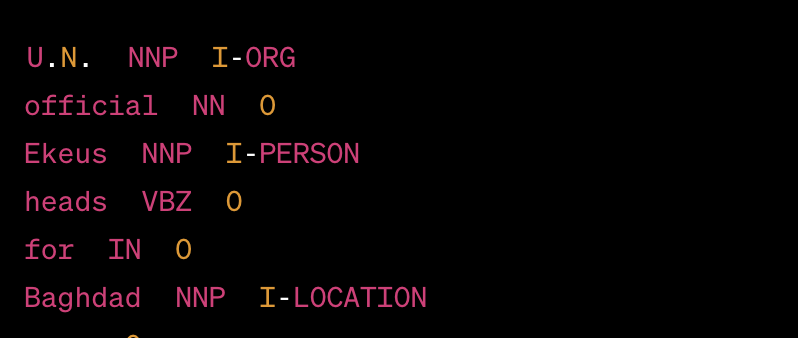
\includegraphics[width=10cm]{conll.png}
\end{center}
\caption{CoNLL2003 dataset}
\label{pic2}
\end{figure}

Poimenovane entitete so razdeljene v štiri glavne kategorije:
\begin{enumerate}
 \item Oseba (PER): Posamezna imena ljudi.
 \item Organizacija (ORG): Imena podjetij, ustanov ali organizacij.
 \item Lokacija (LOC): Imena geografskih lokacij, kot so mesta, države ali regije.
 \item Razno (MISC): Druge poimenovane entitete, ki ne spadajo v zgoraj navedene kategorije, na primer datumi, odstotki ali denar.
 \end{enumerate}
 Podatki v datasetu so predstavljeni v obliki ene besede na vrstico, kjer vsaka vrstica predstavlja besedo in pripadajočo oznako v stavku. Besede in oznake so ločene z presledkom.
 Dataset CoNLL 2003 se pogosto uporablja za evalvacijo zmogljivosti modelov za prepoznavanje poimenovanih entitet in že več let je standardni "benchmark" za raziskovalce in strokovnjake v skupnosti obdelave naravnega jezika. Ostaja dragocen vir za razvoj in preizkušanje novih algoritmov in sistemov za NER. \cite{conll}


CoNLL2003  podatkovna zbirka je običajno razdeljena na tri sklope:
\begin{enumerate}
 \item učni (train) z 14.000 vrsticami  primerov
 \item validacijski (validation) z 3.250 vrsticami primerov
 \item preizkusni (test) z 3.450 vrsticami primerov
 \end{enumerate}

\subsection{IMDb Reviews dataset}
\label{sec:imdb}
IMDB podatkovna zbirka, znana tudi kot IMDB Movie Reviews Dataset. Sestavljen iz pregledov filmov, ki so jih prispevali uporabniki na spletni strani IMDb (Internet Movie Database).

Podatki vsebujejo ocene in besedilne komentarje, ki jih je ustvarila skupnost uporabnikov IMDb. Vsak pregled vsebuje besedilni komentar in oceno filma, ki se giblje med 1 (najslabša) in 10 (najboljša). Cilj te podatkovne zbirke v naravnem jeziku je razviti modele, ki lahko avtomatsko analizirajo besedilne komentarje in napovedo, ali je pregled pozitiven ali negativen glede na oceno in besedilo. \cite{imdb}

IMDB podatkovna zbirka je običajno razdeljena na dva sklopa: 
\begin{enumerate}
 \item učni (train) z 25.000 vrsticami  primerov
 \item preizkusni (test) z 25.000 vrsticami primerov
 \end{enumerate}
Vsak sklop vsebuje tisoče pregledov filmov. To je idealna podatkovna zbirka za naloge analize čustvenega tona besedil (sentiment analysis), kjer modeli ocenjujejo, ali je mnenje v besedilu pozitivno, negativno ali nevtralno.

\subsection{ COCO dataset}
\label{sec:coco}
COCO (Common Objects in Context) je široko uporabljen nabor podatkov v področju računalniškega vida in zaznave objektov. Namenjen je zagotavljanju celovite in raznolike zbirke slik za različne naloge, vključno z zaznavo objektov, segmentacijo in podnaslavljanjem. Nabor podatkov naj bi odražal scenarije iz resničnega sveta in vsebuje slike, ki so kompleksne ter vključujejo več objektov v različnih kontekstih.

Nabor podatkov COCO je obsežen in vsebuje deset tisoče slik z milijoni označenih posameznih objektov. Slike prihajajo iz različnih virov, zajemajo raznolike prizore, ozadja, svetlobne pogoje in velikosti objektov.


Tukaj je nekaj ključnih značilnosti nabora podatkov COCO:
\begin{enumerate}
 \item Kategorije slik: Nabor podatkov COCO vsebuje slike, ki zajemajo 80 različnih kategorij objektov, od splošnih objektov, kot so "oseba," "avto" in "pes," do bolj specifičnih objektov, kot so "mobilni telefon," "zobna ščetka" in "zmaj."

 \item Anotacije: Vsaka slika v naboru podatkov COCO je opremljena z oznakami na ravni objekta in koordinatami  okvirja. To pomeni, da je vsak posamezen objekt določene kategorije znotraj slike označen, okoli njega pa je narisano območje z okvirjem, ki označuje njegovo lokacijo. Informacije o anotacijah so ključnega pomena za usposabljanje modelov za detekcijo objektov in segmentacijo.

 \item Segmentacija objektov: Poleg anotacij območja z okviri nabor podatkov COCO prav tako zagotavlja maske segmentacije na ravni slikovnih pik za vsak posamezen objekt. To pomeni, da so objekti ne le lokalizirani z okviri, ampak so natančno določene tudi meje objektov na ravni slikovnih pik. \cite{coco}


 \end{enumerate}
 COCO podatkovna zbirka je običajno razdeljena na dva sklopa: 
\begin{enumerate}
 \item učni (train) z 117.000 primeri
 \item preizkusni (test) z 4.950 primeri
 \end{enumerate}
 
 \subsection{ CNN/Daily Mail Dataset}
 \label{sec:cnn}
 CNN/Daily Mail je zbirka novičarskih člankov skupaj s povzetki, ki se uporablja za usposabljanje in preizkušanje modelov za povzemanje besedil. Ta nabor podatkov vsebuje različne novičarske članke in njihove povzetke, zaradi česar je primeren za naloge abstraktivnega povzemanja, kjer se ustvarijo povzetki v lastnih besedah, ne le izbirajo stavke iz izvornega besedila.
 Nabor podatkov vsebuje na tisoče člankov s pripadajočimi povzetki, kar omogoča raziskovalcem obsežno treniranje in evaluiranje modelov.\cite{cnn}
 
 Tukaj je nekaj ključnih značilnosti nabora podatkov CNN/Daily Mail:
 \begin{enumerate}
  \item Novičarski Članki in Povzetki: Nabor podatkov vsebuje novičarske članke iz medijskih virov, kot sta CNN (Cable News Network) in Daily Mail, skupaj s pripadajočimi povzetki. Ti članki pokrivajo različne teme in dogodke ter so različnih dolžin.
 \item Abstraktno Povzemanje: Vključuje ustvarjanje povzetka v povsem novih besedah. 
  \end{enumerate}
CNN/Daily Mail podatkovna zbirka je običajno razdeljena na tri sklope: 
\begin{enumerate}
 \item učni (train) z 287.000 vrsticami  primerov
 \item validacijski (validation) z 13.400 vrsticami primerov
 \item preizkusni (test) z 11.500 vrsticami primerov
 \end{enumerate}
 
 \subsection{ semeval-2017 dataset}
  \label{sec:semeval}
 SemEval podatkovna zbirka je zbirka besedilnih podatkov, ki je anotirana za različne naloge na področju obdelave naravnega jezika.
 
Tukaj je nekaj ključnih značilnosti SemEval podatkovnih zbirk:
\begin{enumerate}
 \item Anotacije: Podatki v SemEval podatkovnih zbirkah so običajno anotirani, kar pomeni, da so označeni z dodatnimi informacijami. Na primer, v podatkovni zbirki za naloge razreševanja sentimenta bi bili vzorci besedil označeni s pozitivnimi, negativnimi ali nevtralnimi sentimenti.

 \item Raznolikost: SemEval podatkovne zbirke zajemajo širok spekter nalog, jezikov in domen. To omogoča raziskovalcem primerjavo modelov in pristopov na različnih področjih.

 \end{enumerate}
Raziskovalna skupnost: SemEval podatkovne zbirke so postale pomemben del naravnega jezika raziskovalne skupnosti, saj omogočajo primerjavo najnovejših pristopov in tehnologij na enotnem naboru podatkov. \cite{semeval}



SemEval  podatkovna zbirka je običajno razdeljena na tri sklope: 
\begin{enumerate}
 \item učni (train) z 49.547 vrsticami  primerov
 \item validacijski (dev) z 12.285 vrsticami primerov
 \item preizkusni (test) z 12.285 vrsticami primerov
 \end{enumerate}
 
 %----------------------------------------------------------------
% Poglavje (Uporabljeni korpusi) 6
%----------------------------------------------------------------
\chapter{Metrike}
\label{ch6}

\section{Opis spemenljivk za izračun metrik}
\textbf{Pravilno pozitivni (True Positive)}

Je izraz, ki se uporablja v statistiki in strojnem učenju za opis primerov, kjer je model pravilno napovedal pozitiven rezultat za določeno skupino. To pomeni, da je model prepoznal pozitiven pojav, ko je bil dejansko prisoten. \cite{truevsfalse}

\emph{Primer:}

Predpostavimo, da razvijamo model za prepoznavanje spam sporočil v elektronski pošti. Model pravilno prepozna 25 sporočil kot nezaželena (spam), ki dejansko vsebujejo nezaželeno vsebino. To pomeni, da imamo 25 primerov "pravih pozitivnih". Te primere model pravilno prepozna kot spam, ker resnično vsebujejo neželeno vsebino.





\textbf{Napačno pozitivni (False Positive)}

Označuje situacijo, ko model napačno napove, da je nekaj pozitivno, medtem ko je v resnici negativno. Gre za vrsto napake, kjer model napačno identificira primer kot pripadajoč pozitivnemu razredu, čeprav dejansko pripada negativnemu razredu.\cite{truevsfalse}


\emph{Primer:}

Predpostavimo, da imamo model za prepoznavanje spam sporočil v elektronski pošti. Če model označi sporočilo kot "spam", čeprav ni dejansko spam, imamo situacijo lažno pozitivnega primera. Drugače povedano, model je napačno napovedal pozitiven primer (spam), ko je dejansko negativen primer (ni spam). 





\textbf{Napačno negativni (False Negatives)}

Označuje napako, ki se pojavi v kontekstu klasifikacije ali analize besedila, ko model napačno napove, da je nekaj negativno, čeprav je v resnici pozitivno. To je vrsta napake, kjer model spregleda ali ne prepozna pozitivnih primerov. 
V primeru analize besedila v naravni jezikovni obdelavi, false negative se zgodi, ko model ne uspe zaznati pozitivnega elementa v besedilu, ki bi ga moral prepoznati. Na primer, če imamo model za prepoznavanje pozitivnih izjav v komentarjih in model spregleda pozitivno izjavo, to bi bil primer false negative. \cite{truevsfalse}

\emph{Primer:}


Predpostavimo, da imamo napreden sistem za filtriranje neželenih sporočil (spam), ki ga uporabljamo za preverjanje prihajajočih e-poštnih sporočil. Sistem je zasnovan tako, da prepoznava in premika neželena sporočila v mapo za neželeno pošto.

Vendar pa se pojavi napačno negativen rezultat, ko sistem napačno presodi e-poštno sporočilo kot varno (ne-spam), čeprav vsebuje vse znake neželene vsebine. Na primer, če e-poštno sporočilo vsebuje povezave do nerealnih ponudb ali oglasev za sumljive izdelke, bi bila takšna sporočila številčno gledano ena od "False Negatives".

V tem primeru je sistem spregledal prepoznavo neželene vsebine, kar je povzročilo, da je sporočilo pristalo v glavnem predalu prejete pošte namesto v mapi za neželeno pošto. To lahko predstavlja težavo, saj se takšni neželeni vsebini lahko izognemo le, če sistem zanesljivo prepozna vse takšne primere. \cite{truevsfalse}


\section{Natančnost (Precision)}

Natančnost je pomembna metrika za ocenjevanje uspešnosti modelov v različnih nalogah. Povdarja natančnost pozitivnih napovedi, torej tistih primerov, ki jih model prepozna kot pozitivne. Visoka preciznost pomeni, da so pozitivne napovedi modela zanesljive in imajo malo lažno pozitivnih napak.

V kontekstu naravne jezikovne obdelave, natančnost igra ključno vlogo pri razumevanju besedila. Na primer, pri analizi sentimenta želimo natančno ugotoviti, ali je izraz pozitiven ali negativen. Visoka preciznost v tem primeru pomeni, da so napovedi modela o sentimentu točne in se malo zmotijo.\cite{percision}

 
 Formula za izračun:
\begin{center}
  \Large{Natančnost = \(\frac{True Positive}{True Positive + False Negatives}\)}
\end{center}


\section{Odzivnost (Recall)}
Nanaša se na eno od metrik uspešnosti pri vrednotenju modelov za obdelavo naravnega jezika. Meri kot razmerje med številom pravilno prepoznanih relevantnih primerov in celotnim številom dejansko obstoječih relevantnih primerov. Višja odzivnost pomeni, da je model bolje usposobljen za iskanje in pridobivanje vseh relevantnih informacij, vendar to lahko vodi tudi v več lažno pozitivnih rezultatov. Zato je pomembno doseči uravnoteženost med odzivnostjo in natančnostjo (precision) pri oceni uspešnosti modelov. Primer uporabe odzivnosti  je v iskalnih sistemih, kjer želimo zagotoviti, da se relevantni dokumenti ali informacije ne izpustijo pri iskanju. S pravilno optimizacijo modelov lahko dosežemo visoko kakovostno izluščevanje informacij iz besedil, kar je ključno za številne aplikacije, kot so avtomatizirano odzivanje na povratne informacije strank, analiza sentimenta in razumevanje besedil v različnih jezikih. \cite{percision}

 Formula za izračun:
\begin{center}
 \Large{Odzivnost = \(\frac{True Positive}{True Positive + False Positive}\)}
\end{center}

\section{F1 ocena (F1-score)}

F1 ocena je pomembna metrika za ocenjevanje uspešnosti modelov v obdelavi besedil. Združuje natančnost in odzivnost v eno metriko, ki odraža ravnotežje med tema dvema metrikama. Pri  nalogah, kot so klasifikacija besedil, luščenje informacij ali identifikacija entitet, sta tako natančnost  kot odzivnost ključni. Visoka natančnost pomeni pravilno identifikacijo relevantnih elementov, medtem ko visoka odzivnost zagotavlja prepoznavanje vseh resnično pozitivnih primerov. Izračuna se kot povprečje med natančnost in odzivnost, dajeta pa ji enako težo. To omogoča, da ocenimo, kako dobro model obvladuje oba cilja hkrati. Visoka vrednost F1 ocena kaže, da je model uspešno uskladil identifikacijo pravih pozitivnih primerov z izogibanjem napačno pozitivnim rezultatom. Uporaba metrike je zlasti smiselna, ko sta metriki natančnost in odzivnost pomembni za končni rezultat in ko želimo doseči optimalno uravnoteženost med tema dvema vidikoma.


 Formula za izračun:
\begin{center}
 \Large{F1 ocena = 2 x \(\frac{Natancnost \times Odzivnost}{Natancnost + Odzivnost}\)}
\end{center}

\section{Accuracy}
Accuracy  je metrika, ki se pogosto uporablja za ocenjevanje uspešnosti modelov v strojnem učenju, vključno z modeli uporabljenimi v obdelavi naravnega jezika. Ta metrika meri, kako pravilno model napove razrede ali kategorije za vhodne podatke v primerjavi z dejanskimi vrednostmi.

V kontekstu obdelave naravnega jezika se natančnost uporablja, na primer, pri nalogah klasifikacije besedil. Predpostavimo, da imamo model, ki se uči razvrščati besedila v določene kategorije, kot so "pozitivno", "negativno" ali "neutralno." Za vsako besedilo ima model svojo napoved, kateri kategoriji pripada.\cite{accuracy}

 Formula za izračun:
\begin{center}
  \large{Accuracy = \(\frac{True Positive + True Negative}{True Positive + True Negative +False Positive + False Negative}\)}
\end{center}

\section{ROUGE}
ROUGE je metrika, ki se uporablja za ocenjevanje kakovosti generiranih besedil v primerjavi z referenčnimi besedili. Gre za kratico, ki označuje "Recall-Oriented Understudy for Gisting Evaluation". Metrika ROUGE je pogosto uporabljena v področju obdelave naravnega jezika, še posebej v nalogah avtomatskega povzemanja besedil.

Primerja generirano besedilo z referenčnim besedilom (običajno človeško ustvarjenim besedilom) in oceni, kako dobro so se ujemale. Metrika upošteva različne vidike, kot so prekrivanje besed, besedni nizi in skupna dolžina besedil. Glavni cilj metrike je merjenje stopnje, do katere je generirano besedilo sposobno pravilno povzeti pomembne informacije iz referenčnega besedila.

Obstajajo različne različice metrike ROUGE, kot so ROUGE-1, ROUGE-2, ROUGE-L itd. Vsaka različica meri različne vidike podobnosti med generiranim besedilom in referenčnim besedilom. Na primer, ROUGE-1 meri prekrivanje eno-besednih nizov med generiranim in referenčnim besedilom, medtem ko ROUGE-2 meri prekrivanje dvo-besednih nizov.

Metrika ima širok nabor uporabe v raziskavah in nalogah, ki vključujejo avtomatsko povzemanje besedil, strojno prevajanje in druge naloge, kjer je pomembno oceniti kakovost generiranih besedil v primerjavi z referenčnimi besedili. Metrika lahko pomaga raziskovalcem in razvijalcem oceniti učinkovitost svojih modelov in tehnik ter izboljšati rezultate pri generiranju besedil.


  %----------------------------------------------------------------
% Poglavje (Analiza raziskave) 6
%----------------------------------------------------------------
\chapter{Analiza raziskave}
\label{ch7}
Pri analizi raziskave so bili izbrani trije največji ponudniki storitev v oblaku: Google Cloud, Amazon Web Services ter Microsoft Azure. Pri izbiri odprtokodne rešitve je bilo težko izbrati najboljšega, saj so v tem času tri najboljše odprtokodne rešitve zelo tesno skupaj kakor tudi povezane. Na podlagi pregledanih funkcionalnosti ter uporabe je bil izbran Hugging Face - Transformers. Pomembno je omeniti, da so vse oblačne storitve po rezultatih tesno skupaj v nekaterih primerih, kot je razvidno iz tabele analize je za  klasifikacijo besedila  odprtokodna rešitev Transformers je imela najboljši rezultat. 

\textbf{Analiza napak}


Pri raziskovanju modelov in ter “datasetov”, hitro spoznamo da so lahko modeli celo preveč prilagojeni(overfit) določenemu področju, kar pomeni da preveč podrobno pozna eno področje, na katerem je bil model treniran in ne more dobro generalizirati novih podatkov/primerov, kakor tudi da so premalo podrobni ali premalo raznoliki. 

Zato so najbolj poznani in razširjeni modeli, učeni na širokem naboru različnih podatkov, da je možnost napake manjša. 

 

Vrste napak, ki jih lahko prepoznamo pri NLP modelih: 

Nezadostni podatki: Za gradnjo natančnega modela je potrebna velika količina podatkov. Če ni dovolj podatkov, bo model morda težko naučil vzorce v podatkih. 

Nezadostna raznolikost podatkov: Pomembno je, da imajo podatki za usposabljanje dobro razpršenost. Če so podatki preveč homogeni, bo model morda težko naučil vzorce, ki veljajo za splošne primere. 

Nekvalitetni podatki: Pomembno je, da so podatki za usposabljanje kakovostni. Če so podatki napačni ali pristranski, bo model morda težko naučil natančen model. 

Napačen algoritem: Obstaja veliko različnih algoritmov za stojno učenje, zato je pomembno, da izberete algoritem, ki je primeren za specifično nalogo. Če izberete napačen algoritem, bo morda težko zgraditi natančen model. 

Napačna nastavitev parametrov: Večina algoritmov stojnega učenja ima parametre, ki jih je mogoče prilagoditi za izboljšanje natančnosti modela. Če niso pravilno nastavljeni parametri, bo morda težko zgraditi natančen model. 
NER napake  

Nepravilna identifikacija entitete: To je najpogostejša vrsta napake, ki se pojavi pri poimenovanju entitete. Napaki se lahko zgodijo zaradi številnih razlogov, kot so: 

 

Ime se ne ujema z nobenim od modelov, ki se uporabljajo za poimenovanje entitete. 

Ime je nepravilno zapisano, tako da se uporabljajo majhne črke, zapletene besede ali tuje besede. To lahko oteži identifikacijo imena in njegovo kategorizacijo. 

Ime je zapleteno ali dvoumno zato, ker imajo zapletena imena lahko več kot eno pomensko področje. 

Nepravilna kategorizacija entitete: Ta vrsta napake se pojavi, ko poimenovanje entitete pravilno identificira ime, vendar ga napačno kategorizira. To lahko povzroči, da poimenovanje entitete ne bo uporabno za namen, za katerega je bil namenjen. 

Napaka v kontekstu: Ta vrsta napake se pojavi, ko poimenovanje entitete pravilno identificira ime in ga pravilno kategorizira, vendar ga napačno razvrsti v kontekstu. To lahko povzroči, da poimenovanje entitete ne bo uporabno za namen, za katerega je bil namenjen. 

 

Napaka v viru: Ta vrsta napake se pojavi, ko poimenovanje entitete pravilno identificira ime, ga pravilno kategorizira in ga pravilno razvrsti v kontekstu, vendar ga napačno dobi iz vira. To lahko povzroči, da poimenovanje entitete ne bo uporabno za namen, za katerega je bil namenjen. 



 \begin{figure}[h!]
\begin{center}
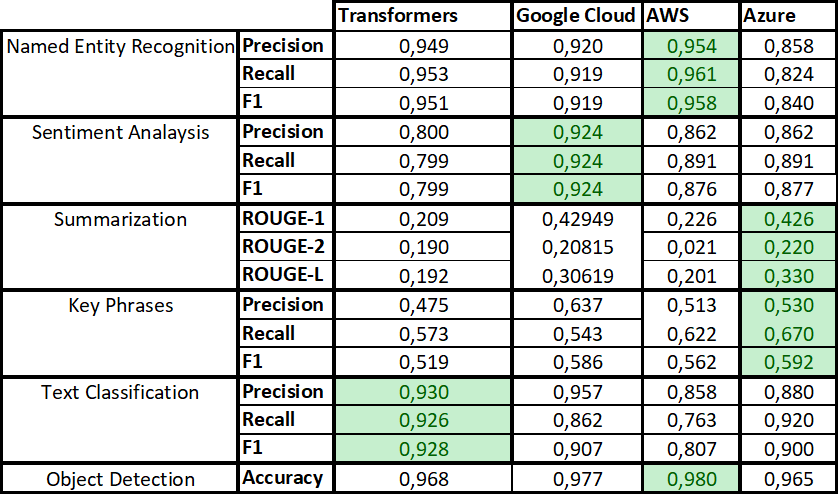
\includegraphics[width=10cm]{tabela.png}
\end{center}
\caption{ Tabela analize (Rezultati so zaokroženi na 3 decimalna mesta)}
\label{pic2}
\end{figure}

\begin{table}[t!]
\centering
\caption{Tabela analize (Rezultati so zaokroženi na 3 decimalna mesta)}
\label{my-label}
\resizebox{\textwidth}{!}{%
\begin{tabular}{lrrrrrr}
\hline
\multicolumn{1}{r}{} &   & \textbf{Transformers}             & \textbf{Vertex AI}                & \textbf{SageMaker}               & \textbf{Cognitive Services}                             \\ \hline                                                                                                                                                                                                                                                                                                                                           
\textbf{Prepoznavanje imenskih entitet}                         & Natančnost  & 16.274                & 332                  & 16.274               & -6.521                                         \\
				&  Odzivnost.  & 1.088                & 332                  & 16.274               & -6.521    \\
                                 & F1 ocena    & 1.088                & 332                  & 16.274               & -6.521    \\

\textbf{Analiza sentimenta}                           & Natančnost  & 193.815              & 188.888              & 506.999              & 15.074                                            \\
                       &  Odzivnost & 193.815              & 188.888              & 506.999              & 15.074                                            \\
                        & F1 ocena   & 193.815              & 188.888              & 506.999              & 15.074                                            \\
\textbf{Povzetek} & Natančnost  & 193.815              & 188.888              & 506.999              & 15.074                                            \\
                       &  Odzivnost & 193.815              & 188.888              & 506.999              & 15.074                                            \\
                        & F1 ocena   & 193.815              & 188.888              & 506.999              & 15.074     \\
\textbf{Izvleček besedne zveze}   & Natančnost  & 193.815              & 188.888              & 506.999              & 15.074                                            \\
                       &  Odzivnost & 193.815              & 188.888              & 506.999              & 15.074                                            \\
                        & F1 ocena   & 193.815              & 188.888              & 506.999              & 15.074     \\       
\textbf{Klasifikacija besedila} & Natančnost  & 193.815              & 188.888              & 506.999              & 15.074                                            \\
                       &  Odzivnost & 193.815              & 188.888              & 506.999              & 15.074                                            \\
                        & F1 ocena   & 193.815              & 188.888              & 506.999              & 15.074     \\
\textbf{Zaznava objektov} & Natančnost  & 193.815              & 188.888              & 506.999              & 15.074                                            \\
                       &  Odzivnost & 193.815              & 188.888              & 506.999              & 15.074                                            \\
                        & F1 ocena   & 193.815              & 188.888              & 506.999              & 15.074                                                                   
\end{tabular}}
\end{table}

Pri testitranju  imenovanje imenskih entitet je najvišjo uspešnost dosegla storitev AWS Sage Maker. Na drugem mestu se je uvrstila odprtokodna storitev Hugging Face Transformers, medtem ko je tretje mesto zasedla storitev Vertex AI ponudnika Google Cloud.

Pri testiranju sentimentalne analize je najboljše rezultate dosegla storitev AWS SageMaker. Na drugem mestu se je uvrstila odprtokodna rešitev Hugging Face Transformers, medtem ko je tretje mesto zasedla storitev Vertex AI podjetja Google Cloud.

Najboljši rezultati so bili doseženi pri povzemanju z uporabo storitve Azure Cognitive Services. Na drugem mestu se je uvrstil Vertex AI, medtem ko je tretje mesto pripadlo AWS SageMaker.

V ocenjevanju izvlečka besednih zvez je najvišje mesto osvojila storitev Azure Cognitive Services. Na drugem mestu se je uvrstil Vertex AI, medtem ko je tretje mesto zasedel AWS SageMaker.

Pri klasifikaciji besedila se je najboljša učinkovitost pokazala pri odprtokodni platformi Transformers. Na drugem mestu je bila storitev Vertex AI, medtem ko je tretje mesto pripadlo storitvi Azure Cognitive Services.

V zaznavanju objektov je najvišje mesto zasedla storitev AWS Cognitive Services, takoj za njo je sledil Vertex AI, medtem ko je tretje mesto pripadlo odprtokodni rešitvi Transformers.



V nadaljevanju so predstavljeni podrobnejši rezultati treh iteracij  z povprečnimi vrednostmi pripadajočih metrik ter  standardni odklon kateri je merilo razpršenosti podatkov. Pomaga nam razumeti, koliko se podatki razlikujejo od povprečne vrednosti.
\newpage


\section{Prepoznavanje imenskih entitet (Named Entity Recognition)}
\begin{table}[h!]
\centering
\caption{Prepoznavanje imenskih entitet}
\label{my-label}
\resizebox{\textwidth}{!}{%
\begin{tabular}{lrrrrrr}
\hline
\multicolumn{1}{r}{} &   & \textbf{Iteracija 1}             & \textbf{Iteracija 2}                & \textbf{Iteracija 3}               & \textbf{Povprečje}       & \textbf{St. odklon}                         \\ \hline                                                                                                                                                                                                                                                                                                                                           
\textbf{Transformers}   & Odzivnost  & 0.929              & 0.912                  & 0.917              & 0.919  & 0.009                                    \\
				    &  Natančnost  & 0.924              & 0.945                  & 0.901               & 0.923 & 0.022  \\
                                     & F1 ocena    & 0.927                 & 0.928                  & 0.909             & 0.921   & 0.011 \\
\textbf{Google Vertex AI}         & Odzivnost  & 0.946             & 0.914              & 0.896              & 0.919     & 0.025                                        \\
                                   &  Natančnost & 0.895              & 0.923              & 0.942              & 0.920              & 0.024                             \\
                                   & F1 ocena   & 0.920              & 0.918              & 0.918              & 0.919                  & 0.001                          \\
\textbf{Amazon SageMaker}.   & Odzivnost & 0.981              & 0.962              & 0.941              & \textbf{0.961}       & 0.020                                     \\
                                   &  Natančnost & 0.962              & 0.980              & 0.921              & \textbf{0.954}                 & 0.030                             \\
                                   & F1 ocena   & 0.971              & 0.971              & 0.931              & \textbf{0.958}      & 0.023 \\
\textbf{Azure Cognitive Services}   & Odzivnost  & 0.821              & 0.831             & 0.821              & 0.824   & 0.006                                           \\
                       &  Natančnost & 0.831              & 0.841              & 0.903              & 0.858                                   & 0.039        \\
                        & F1 ocena   & 0.826              & 0.836              & 0.860              & 0.841                                    & 0.017                                       
\end{tabular}}
\end{table}

 
 \begin{figure}[h!]
\begin{center}
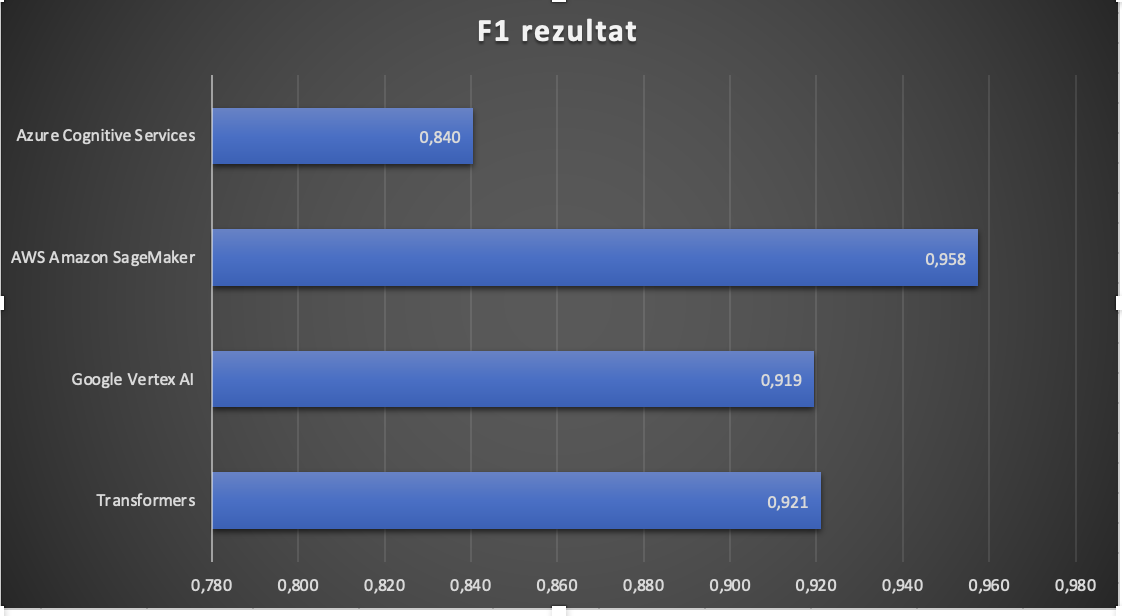
\includegraphics[width=10cm]{NER.png}
\end{center}
\caption{Prepoznavanje imenskih entitet F1 rezultat}
\label{pic2}
\end{figure}

Pri analizi imenskih entitet je bil uporabljen \hyperref[sec:my_subsection]{\underline {CONLL-2003}} dataset.

Za prepoznavanje oseb (PER) in organizacij (ORG) se je najbolje izkazal Vertex AI storitev. Na splošno pa je bil v vseh področjih najboljši AWS SageMaker storitev.

\newpage
\textbf{Analiza napak} 

Najpogosteje opažene napake pri prepoznavi imenskih entitet:  
\begin{enumerate}
 \item Napake imen: To so napake v imenu imenske entitete, na primer napačna črka ali napačen zlog, zapletene besede ali tuje besede. To lahko oteži identifikacijo imena in njegovo kategorizacijo. 
 \item Napake v tipu: napaka v tipu imenske entitete, na primer napačno označitev osebe kot kraja ali obratno. Ime je zapleteno ali dvoumno zato, ker imajo zapletena imena lahko več kot eno pomensko področje. 
 \item Izpuščanje/nekategorizacija: napaka, pri katerih se imenska entiteta izpusti iz besedila. 
 \item Ponavljanje:napaka, pri katerih se imenska entiteta ponovi v besedilu. 
 \end{enumerate}

\newpage
\section{Analiza sentimenta (Sentiment Analaysis)}

\begin{table}[h!]
\centering
\caption{Analiza sentimenta}
\label{my-label}
\resizebox{\textwidth}{!}{%
\begin{tabular}{lrrrrrr}
\hline
\multicolumn{1}{r}{} &   & \textbf{Iteracija 1}             & \textbf{Iteracija 2}                & \textbf{Iteracija 3}               & \textbf{Povprečje}   & \textbf{St. odklon}                           \\ \hline                                                                                                                                                                                                                                                                                                                                           
\textbf{Transformers}   & Odzivnost  & 0.937              & 0.912                 & 0.930              & 0.926                      & 0.013                \\
				    &  Natančnost  & 0.938              & 0.987                  & 0.860               & 0.928                & 0.064                      \\
                                     & F1 ocena    & 0.937                 & 0.952                  & 0.893             & 0.929                  & 0.031   \\
\textbf{Vertex AI}         & Odzivnost  & 0.921              & 0.948              & 0.938              & 0.936                          & 0.014                   \\
                                   &  Natančnost & 0.942             & 0.888              & 0.943              & 0.924                          & 0.031                \\
                                   & F1 ocena   & 0.931            & 0.917            & 0.940              & 0.930                                & 0.012            \\
\textbf{Amazon SageMaker}.   & Odzivnost  & 0.901              & 0.882              & 0.891              & 0.891              & 0.010                               \\
                                   &  Natančnost & 0.821              & 0.853              & 0.912              & 0.862                         & 0.046                   \\
                                   & F1 ocena   & 0.859              & 0.867              & 0.901              & 0.876                            & 0.022                        \\
\textbf{Azure Cognitive Services}   & Odzivnost  & 0.881              & 0.905              & 0.887              & 0.981        & 0.012                                     \\
                       &  Natančnost & 0.852              & 0.884              & 0.851              & 0.862                                      & 0.019       \\
                        & F1 ocena   & 0.866              & 0.894              & 0.869              & 0.876                                        & 0.015                                   
\end{tabular}}
\end{table}

 \begin{figure}[h!]
\begin{center}
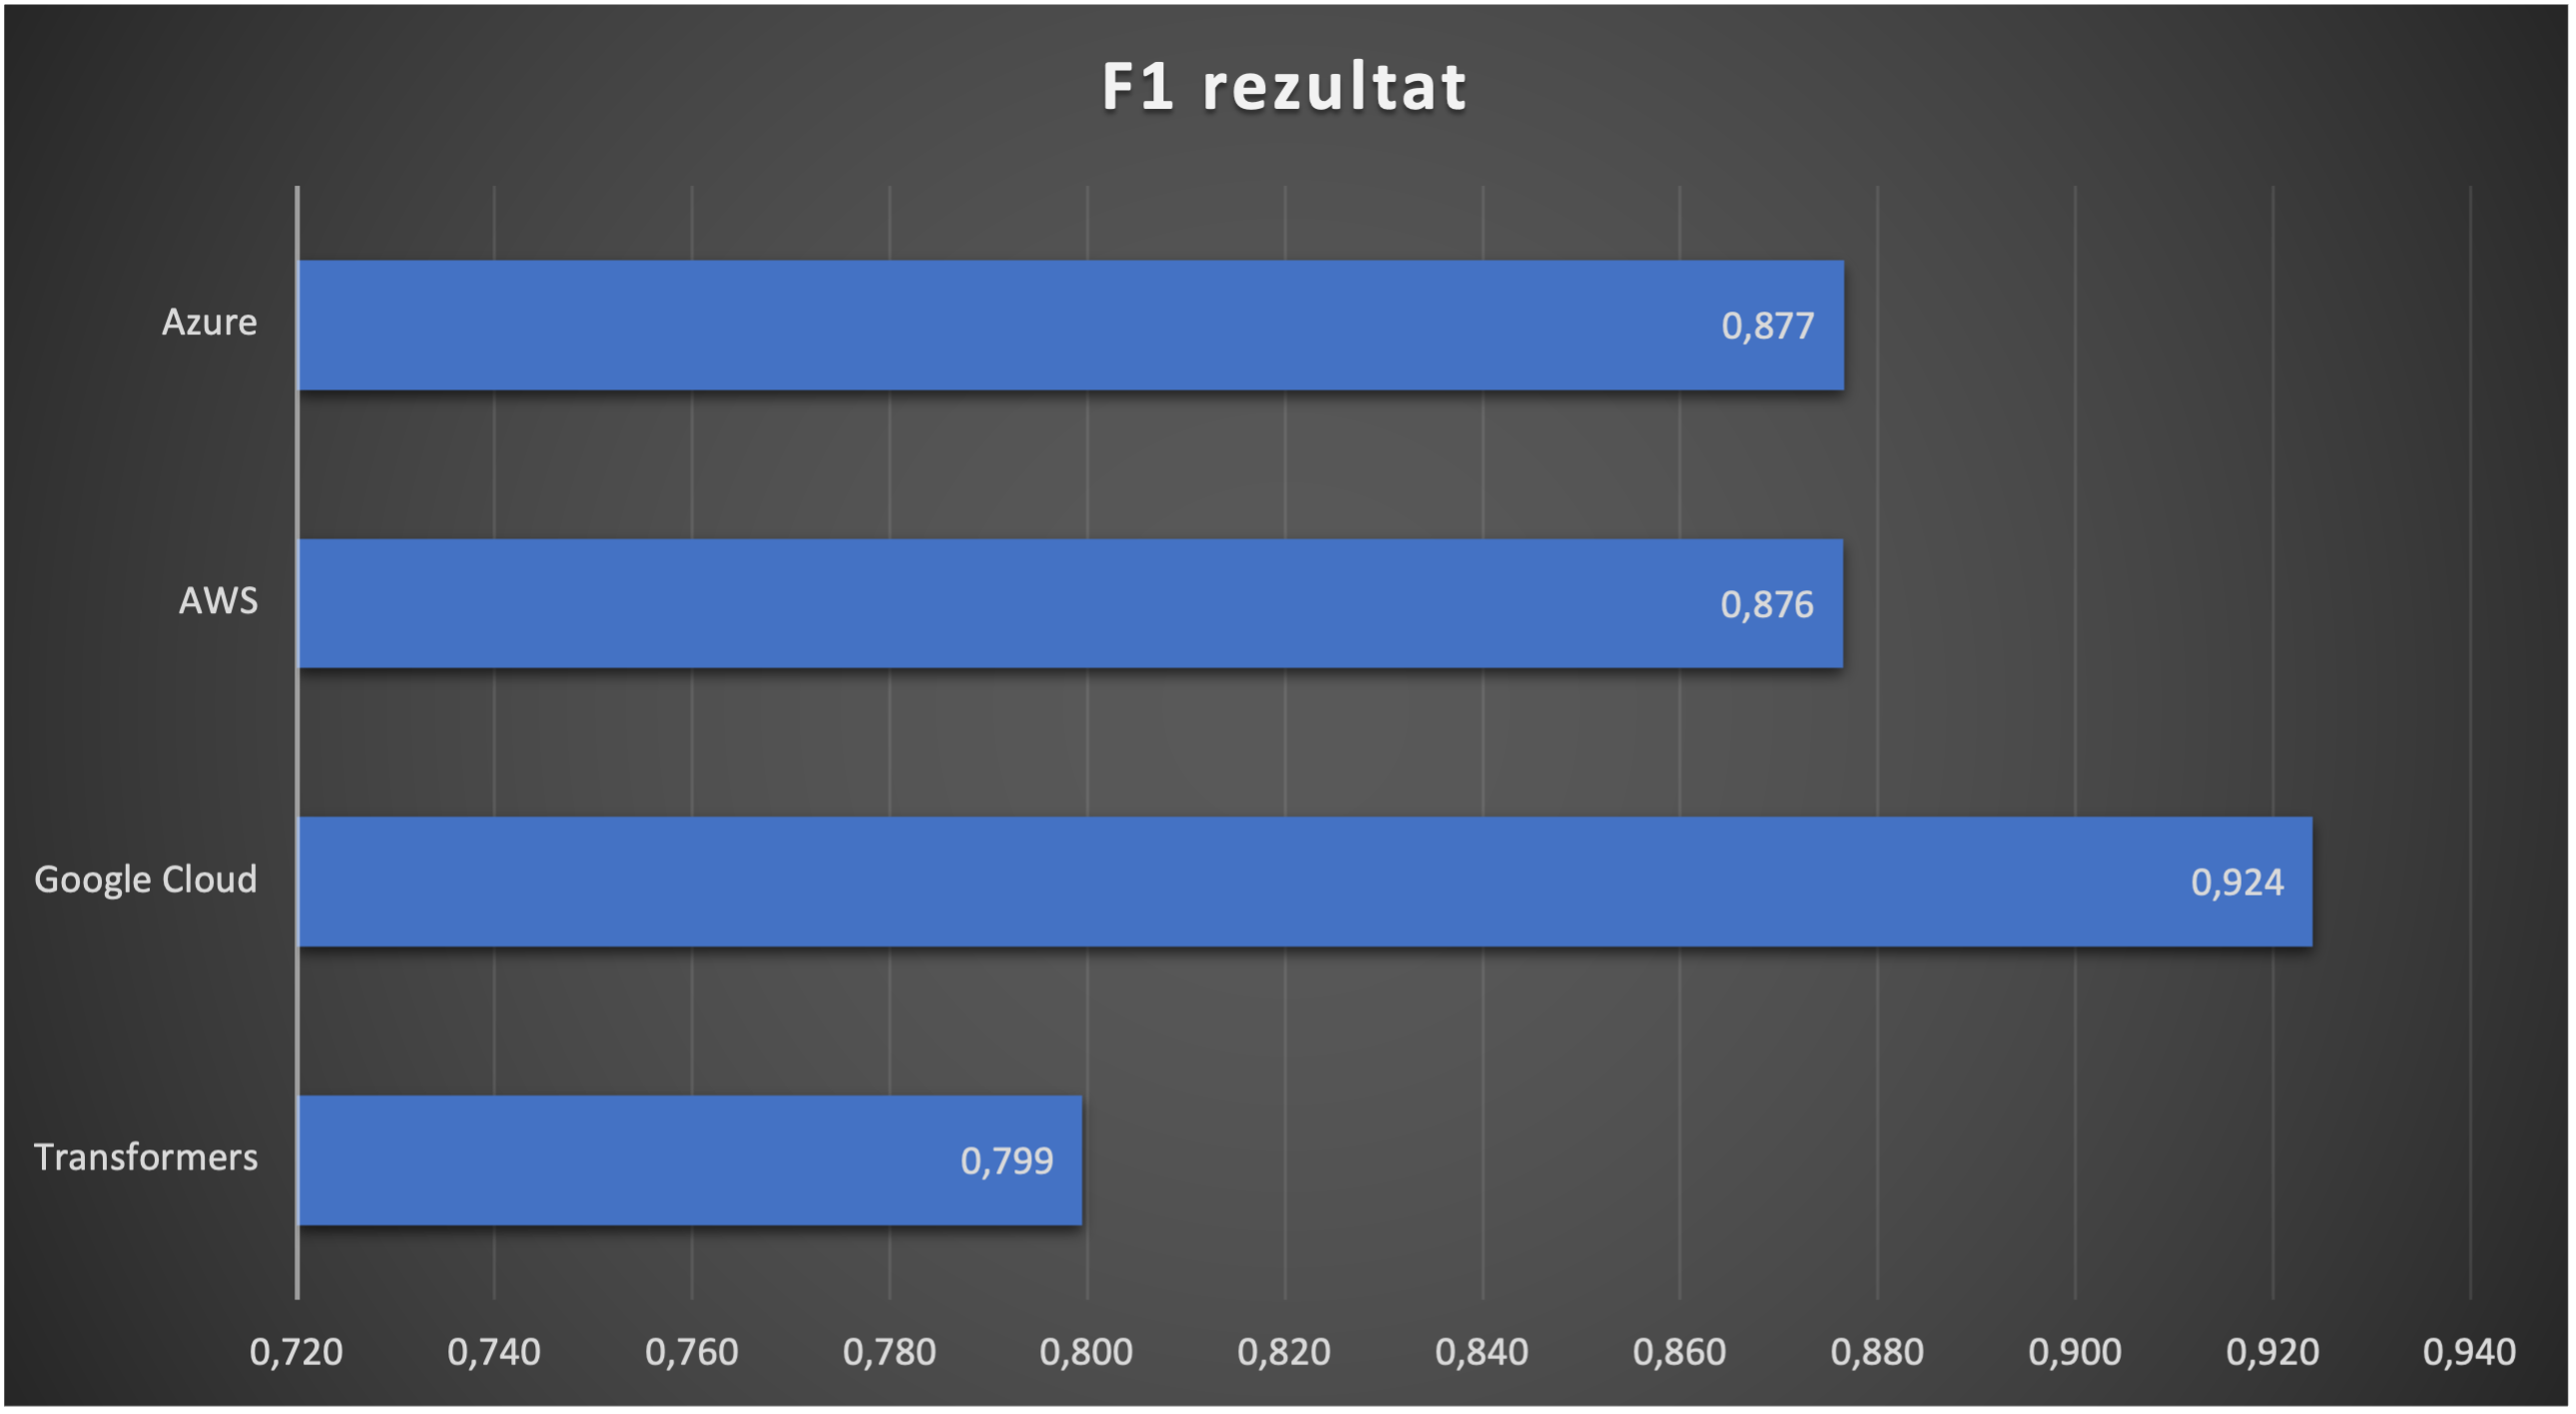
\includegraphics[width=10cm]{KP.png}
\end{center}
\caption{Analiza sentimenta F1 rezultat}
\label{pic2}
\end{figure}
Pri analizi imenskih entitet je bil uporabljen  \hyperref[sec:imdb]{\underline {IMDb Reviews}} dataset.
Za analizo sentimenta  je bila najboljša Vertex AI storitev.

\pagebreak 

\section{Povzetek (Summarisation)}
\begin{table}[h!]
\centering
\caption{Povzetek}
\label{my-label}
\resizebox{\textwidth}{!}{%
\begin{tabular}{lrrrrrr}
\hline
\multicolumn{1}{r}{} &   & \textbf{Iteracija 1}             & \textbf{Iteracija 2}                & \textbf{Iteracija 3}               & \textbf{Povprečje}                             \\ \hline                                                                                                                                                                                                                                                                                                                                           
\textbf{Transformers}   & ROUGE-L   & 0.178              & 0.187                 & 0.212              & 0.192                                     \\
\textbf{Vertex AI}         & ROUGE-L   & 0.312              & 0.291              & 0.315              & 0.306                                           \\
\textbf{Amazon SageMaker}.   & ROUGE-L   & 0.203             & 0.184              & 0.2016             & 0.201                                          \\
\textbf{Azure Cognitive Services}   & ROUGE-L   & 0.387              & 0.318             & 0.284             & 0.330                                                                                                                
\end{tabular}}
\end{table}

 \begin{figure}[h!]
\begin{center}
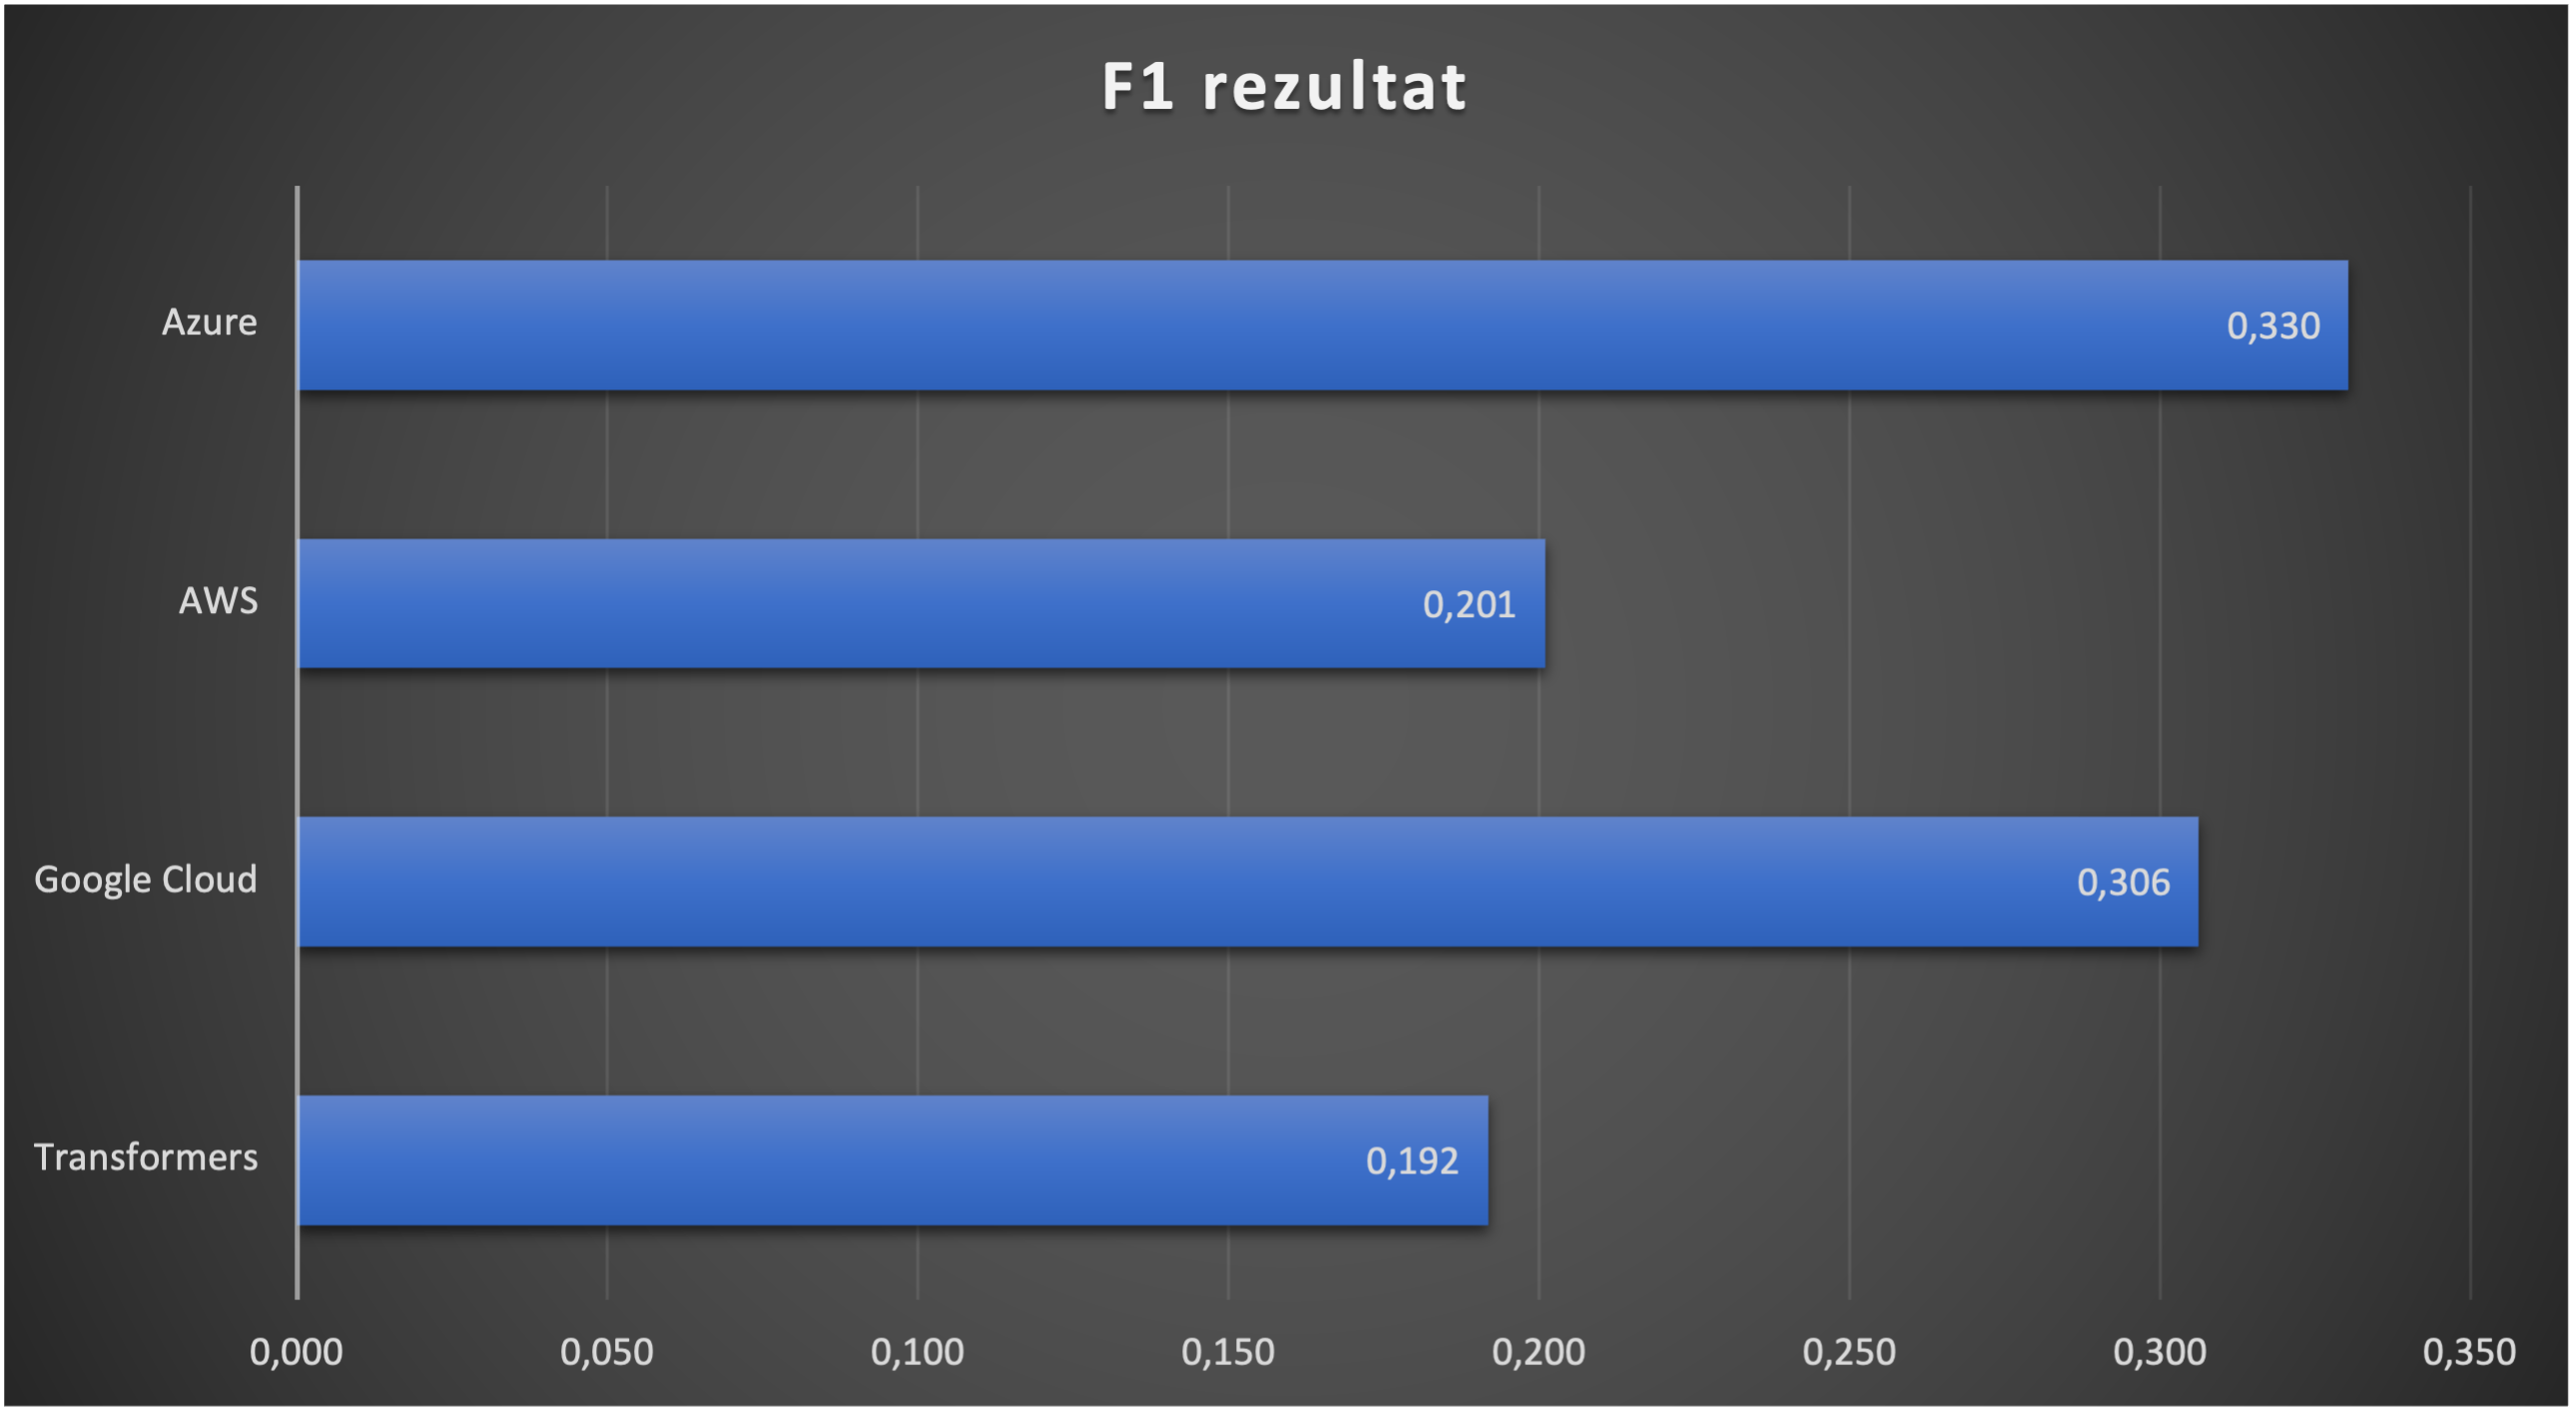
\includegraphics[width=10cm]{SUMM.png}
\end{center}
\caption{Povzetek F1 rezultat}
\label{pic2}
\end{figure}

Pri izdelavi povzetka je bil uporabljen dataset  \hyperref[sec:cnn]{\underline {CNN/Daily Mail}}.

Kot vrhunska izbira za ustvarjanje povzetkov pa se je izkazala storitev Vertex AI.

%----------------------------------------------------------------
%Izvleček besedne zveze 

%----------------------------------------------------------------
  \newpage
\section{Izvleček besedne zveze  (Key Phrases)}


\begin{table}[h!]
\centering
\caption{Izvleček besedne zveze}
\label{my-label}
\resizebox{\textwidth}{!}{%
\begin{tabular}{lrrrrrr}
\hline
\multicolumn{1}{r}{} &   & \textbf{Iteracija 1}             & \textbf{Iteracija 2}                & \textbf{Iteracija 3}               & \textbf{Povprečje}                             \\ \hline                                                                                                                                                                                                                                                                                                                                           
\textbf{Transformers}   & Odzivnost  & 0.523              & 0.640                  & 0.556              & 0.573                                         \\
				    &  Natančnost  & 0.398               & 0.499                 & 0.528               & 0.475    \\
                                     & F1 ocena    & 0.452                  & 0.561                  & 0.542              & 0.519    \\

\textbf{Vertex AI}         & Odzivnost  & 0.499              & 0.541              & 0.589              & 0.543                                            \\
                                   &  Natančnost & 0.688             & 0.635              & 0.589              & 0.637                                            \\
                                   & F1 ocena   & 0.578             & 0.584              & 0.589              & 0.586                                          \\
\textbf{Amazon SageMaker}.   & Odzivnost  & 0.675              & 0.605              & 0.587              & 0.622                                           \\
                                   &  Natančnost & 0.520              & 0.492             & 0.526             & 0.513                                           \\
                                   & F1 ocena   & 0.587             & 0.543             & 0.555              & 0.562    \\
\textbf{Azure Cognitive Services}   & Odzivnost  & 0.532              & 0.559             & 0.500              & 0.530                                           \\
                       &  Natančnost & 0.674              & 0.648             & 0.689              & 0.670                                          \\
                        & F1 ocena   & 0.595              & 0.600              & 0.579              & 0.592                                                                     
\end{tabular}}
\end{table}

 \begin{figure}[h!]
\begin{center}
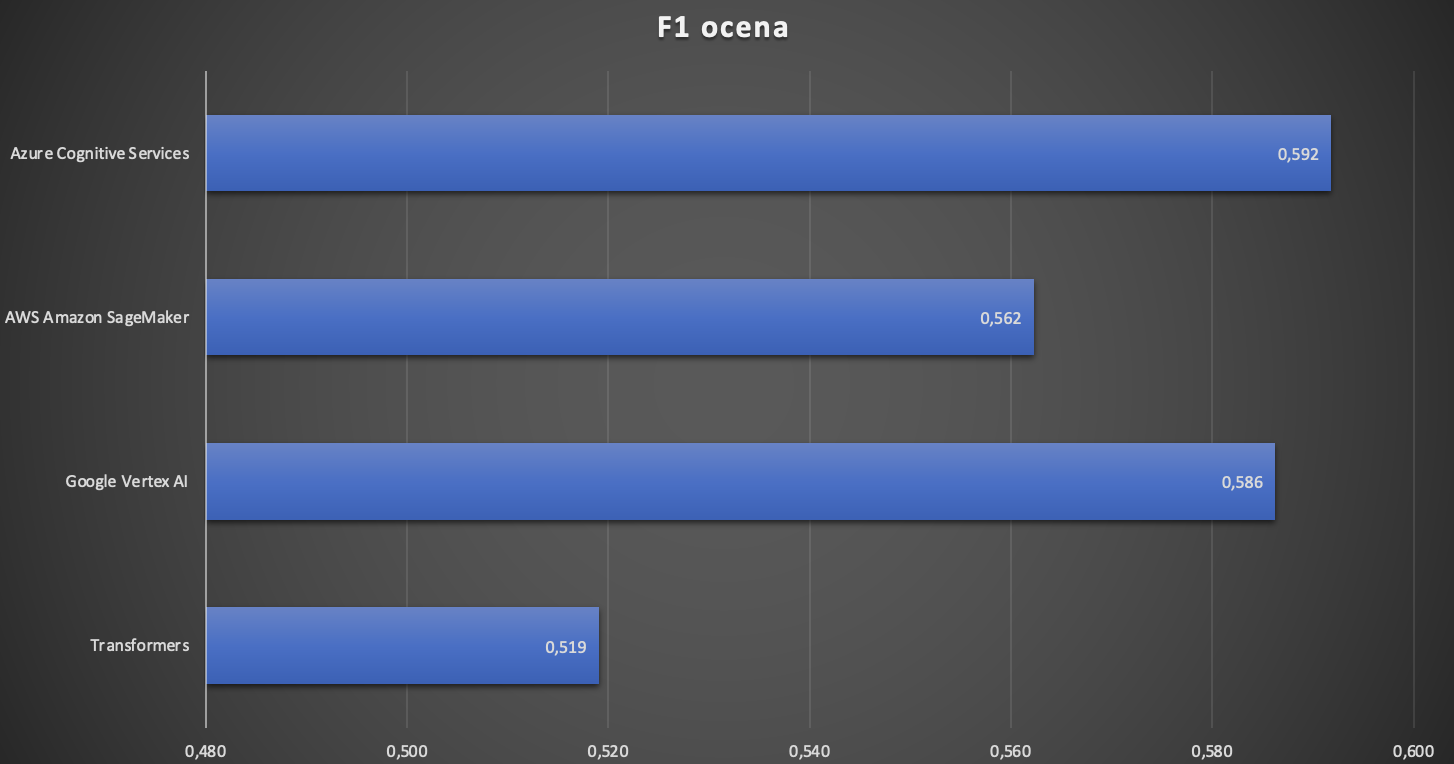
\includegraphics[width=10cm]{KEY.png}
\end{center}
\caption{Izvleček besedne zveze F1 rezultat}
\label{pic2}
\end{figure}

Pri izvajanju naloge zvlečka besedne zveze je bil uporabljen podatkovni niz  \hyperref[sec:semeval]{\underline {semeval-2017}}.

Kot najboljša rešitev za naloge izvlečka besedne zveze pa se je izkazala storitev Azure Cognitive Services.

\pagebreak 
%----------------------------------------------------------------
% Klasifikacija besedila 
%----------------------------------------------------------------

\section{Klasifikacija besedila  (Text Classification)}
\begin{table}[h!]
\centering
\caption{Klasifikacija besedila}
\label{my-label}
\resizebox{\textwidth}{!}{%
\begin{tabular}{lrrrrrr}
\hline
\multicolumn{1}{r}{} &   & \textbf{Iteracija 1}             & \textbf{Iteracija 2}                & \textbf{Iteracija 3}               & \textbf{Povprečje}                             \\ \hline                                                                                                                                                                                                                                                                                                                                           
\textbf{Transformers}   & Odzivnost  & 0.933             & 0.948                  &  0.896             &  0.926                                         \\
				    &  Natančnost  &  0.898               & 0.935                 & 0.958               &  0.930    \\
                                     & F1 ocena    &  0.915                  &  0.941                  &  0.926              &  0.928    \\
\textbf{Vertex AI}         & Odzivnost  &  0.842              &  0.901              &  0.844             &  0.962                                            \\
                                   &  Natančnost &  0.989              &  0.924              &  0.959              &  0.957                                            \\
                                   & F1 ocena   &  0.910              &  0.912              &  0.989              &  0.907                                           \\
\textbf{Amazon SageMaker}.   & Odzivnost  &  0.789              &  0.802             &  0.697              &  0.763                                           \\
                                   &  Natančnost &  0.879              &  0.799              &  0.895              &  0.858                                            \\
                                   & F1 ocena   &  0.832              &  0.800              &  0.784              &  0.808    \\
\textbf{Azure Cognitive Services}   & Odzivnost  &  0.935              &  0.925             &  0.900              &  0.920                                           \\
                       &  Natančnost &  0.827              &  0.888              &  0.925             &  0.880                                            \\
                        & F1 ocena   &  0.878              &  0.906              &  0.912              &  0.900                                                                         
\end{tabular}}
\end{table}

 \begin{figure}[h!]
\begin{center}
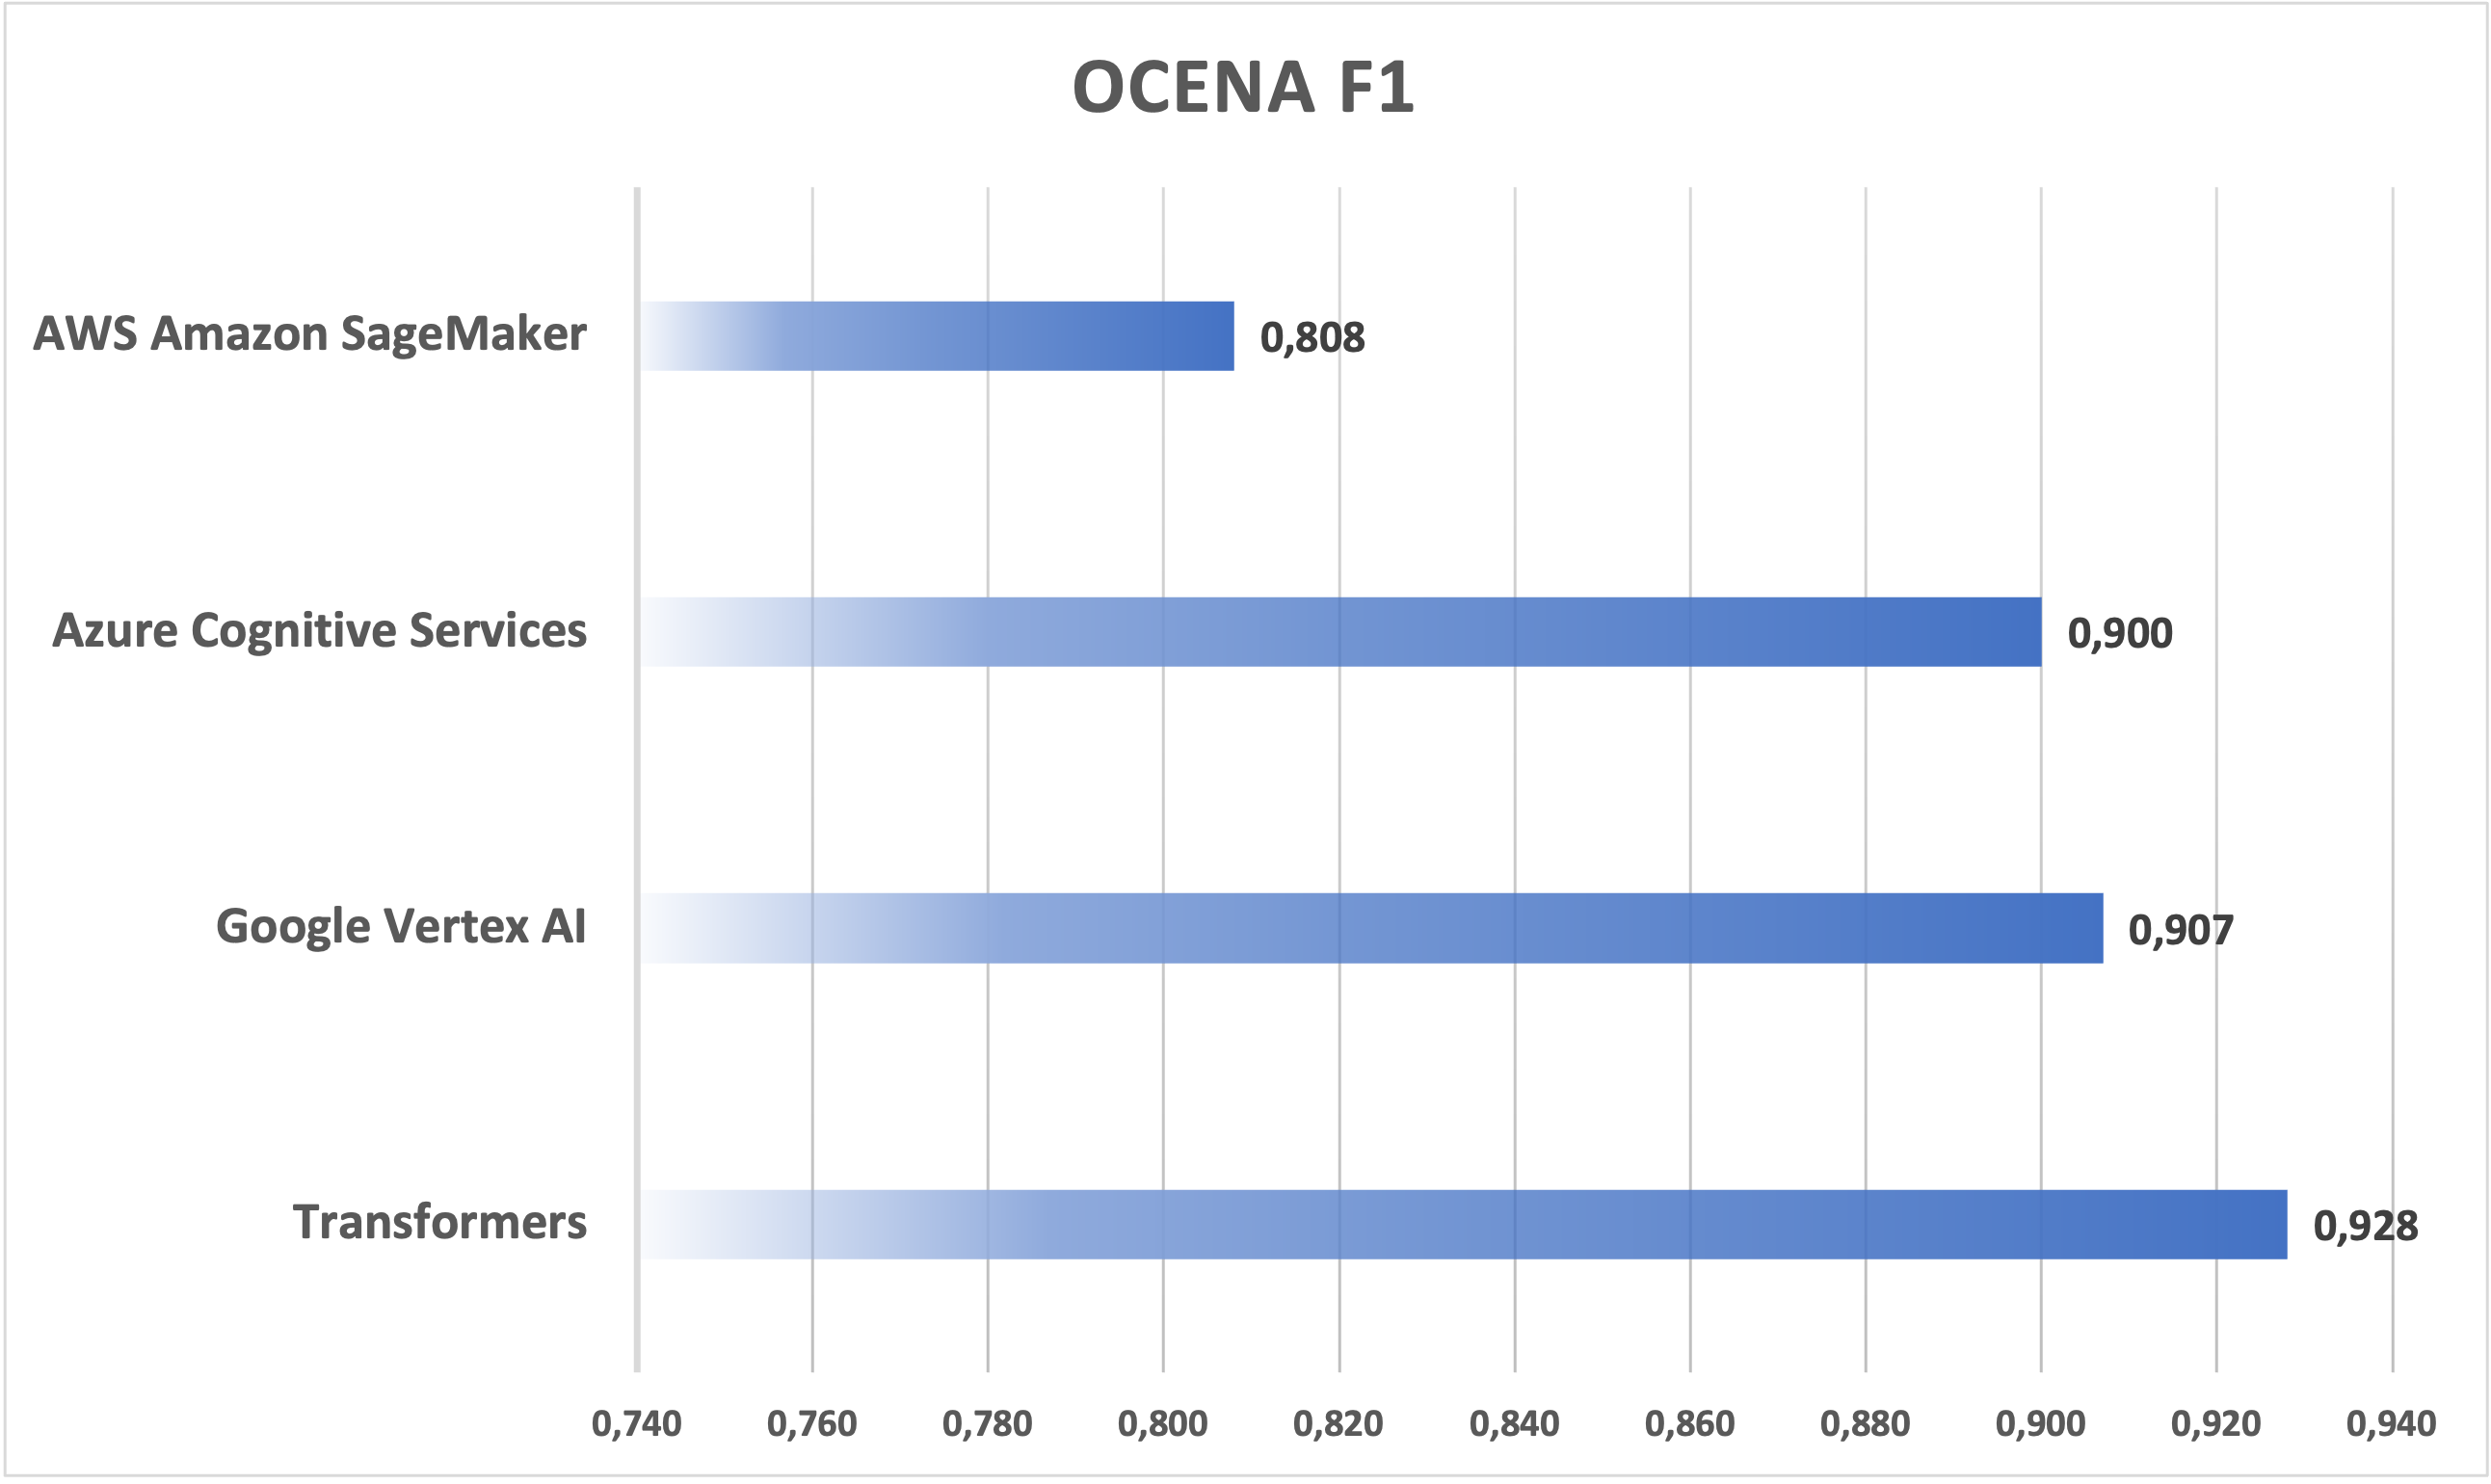
\includegraphics[width=10cm]{CLASSIFICATION.png}
\end{center}
\caption{ Klasifikacija besedila  F1 rezultat}
\label{pic2}
\end{figure}

Pri izvajanju naloge klasifikacije besedila je bil uporabljen podatkovni niz  \hyperref[sec:imdb]{\underline {IMDb Reviews}}.

Kot najboljša rešitev za naloge klasifikacije besedila pa se je izkazala storitev Transformers.

\pagebreak 
%----------------------------------------------------------------
% Zaznava objektov 
%---------------------------------------------------------------

\section{Zaznava objektov  (Object Detection)}
\begin{table}[h!]
\centering
\caption{Zaznava objektov }
\label{my-label}
\resizebox{\textwidth}{!}{%
\begin{tabular}{lrrrrrr}
\hline
\multicolumn{1}{r}{} &   & \textbf{Iteracija 1}             & \textbf{Iteracija 2}                & \textbf{Iteracija 3}               & \textbf{Povprečje }                             \\ \hline                                                                                                                                                                                                                                                                                                                                           
\textbf{Transformers}   & Accuracy  & 0.900             & 0.970                  & 0.940              & 0.940                                      \\
\textbf{Vertex AI}         & Accuracy  & 0.963              & 0.991              & 0.977             & 0.977                                            \\
\textbf{Amazon SageMaker}.   & Accuracy  & 0.995              & 0.963              & 0.982              & 0.980                                            \\
\textbf{Azure Cognitive Services}   & Odzivnost  & 0.960             & 0.950              & 0.985             & 0.965                                                                                   
\end{tabular}}
\end{table}


 \begin{figure}[h!]
\begin{center}
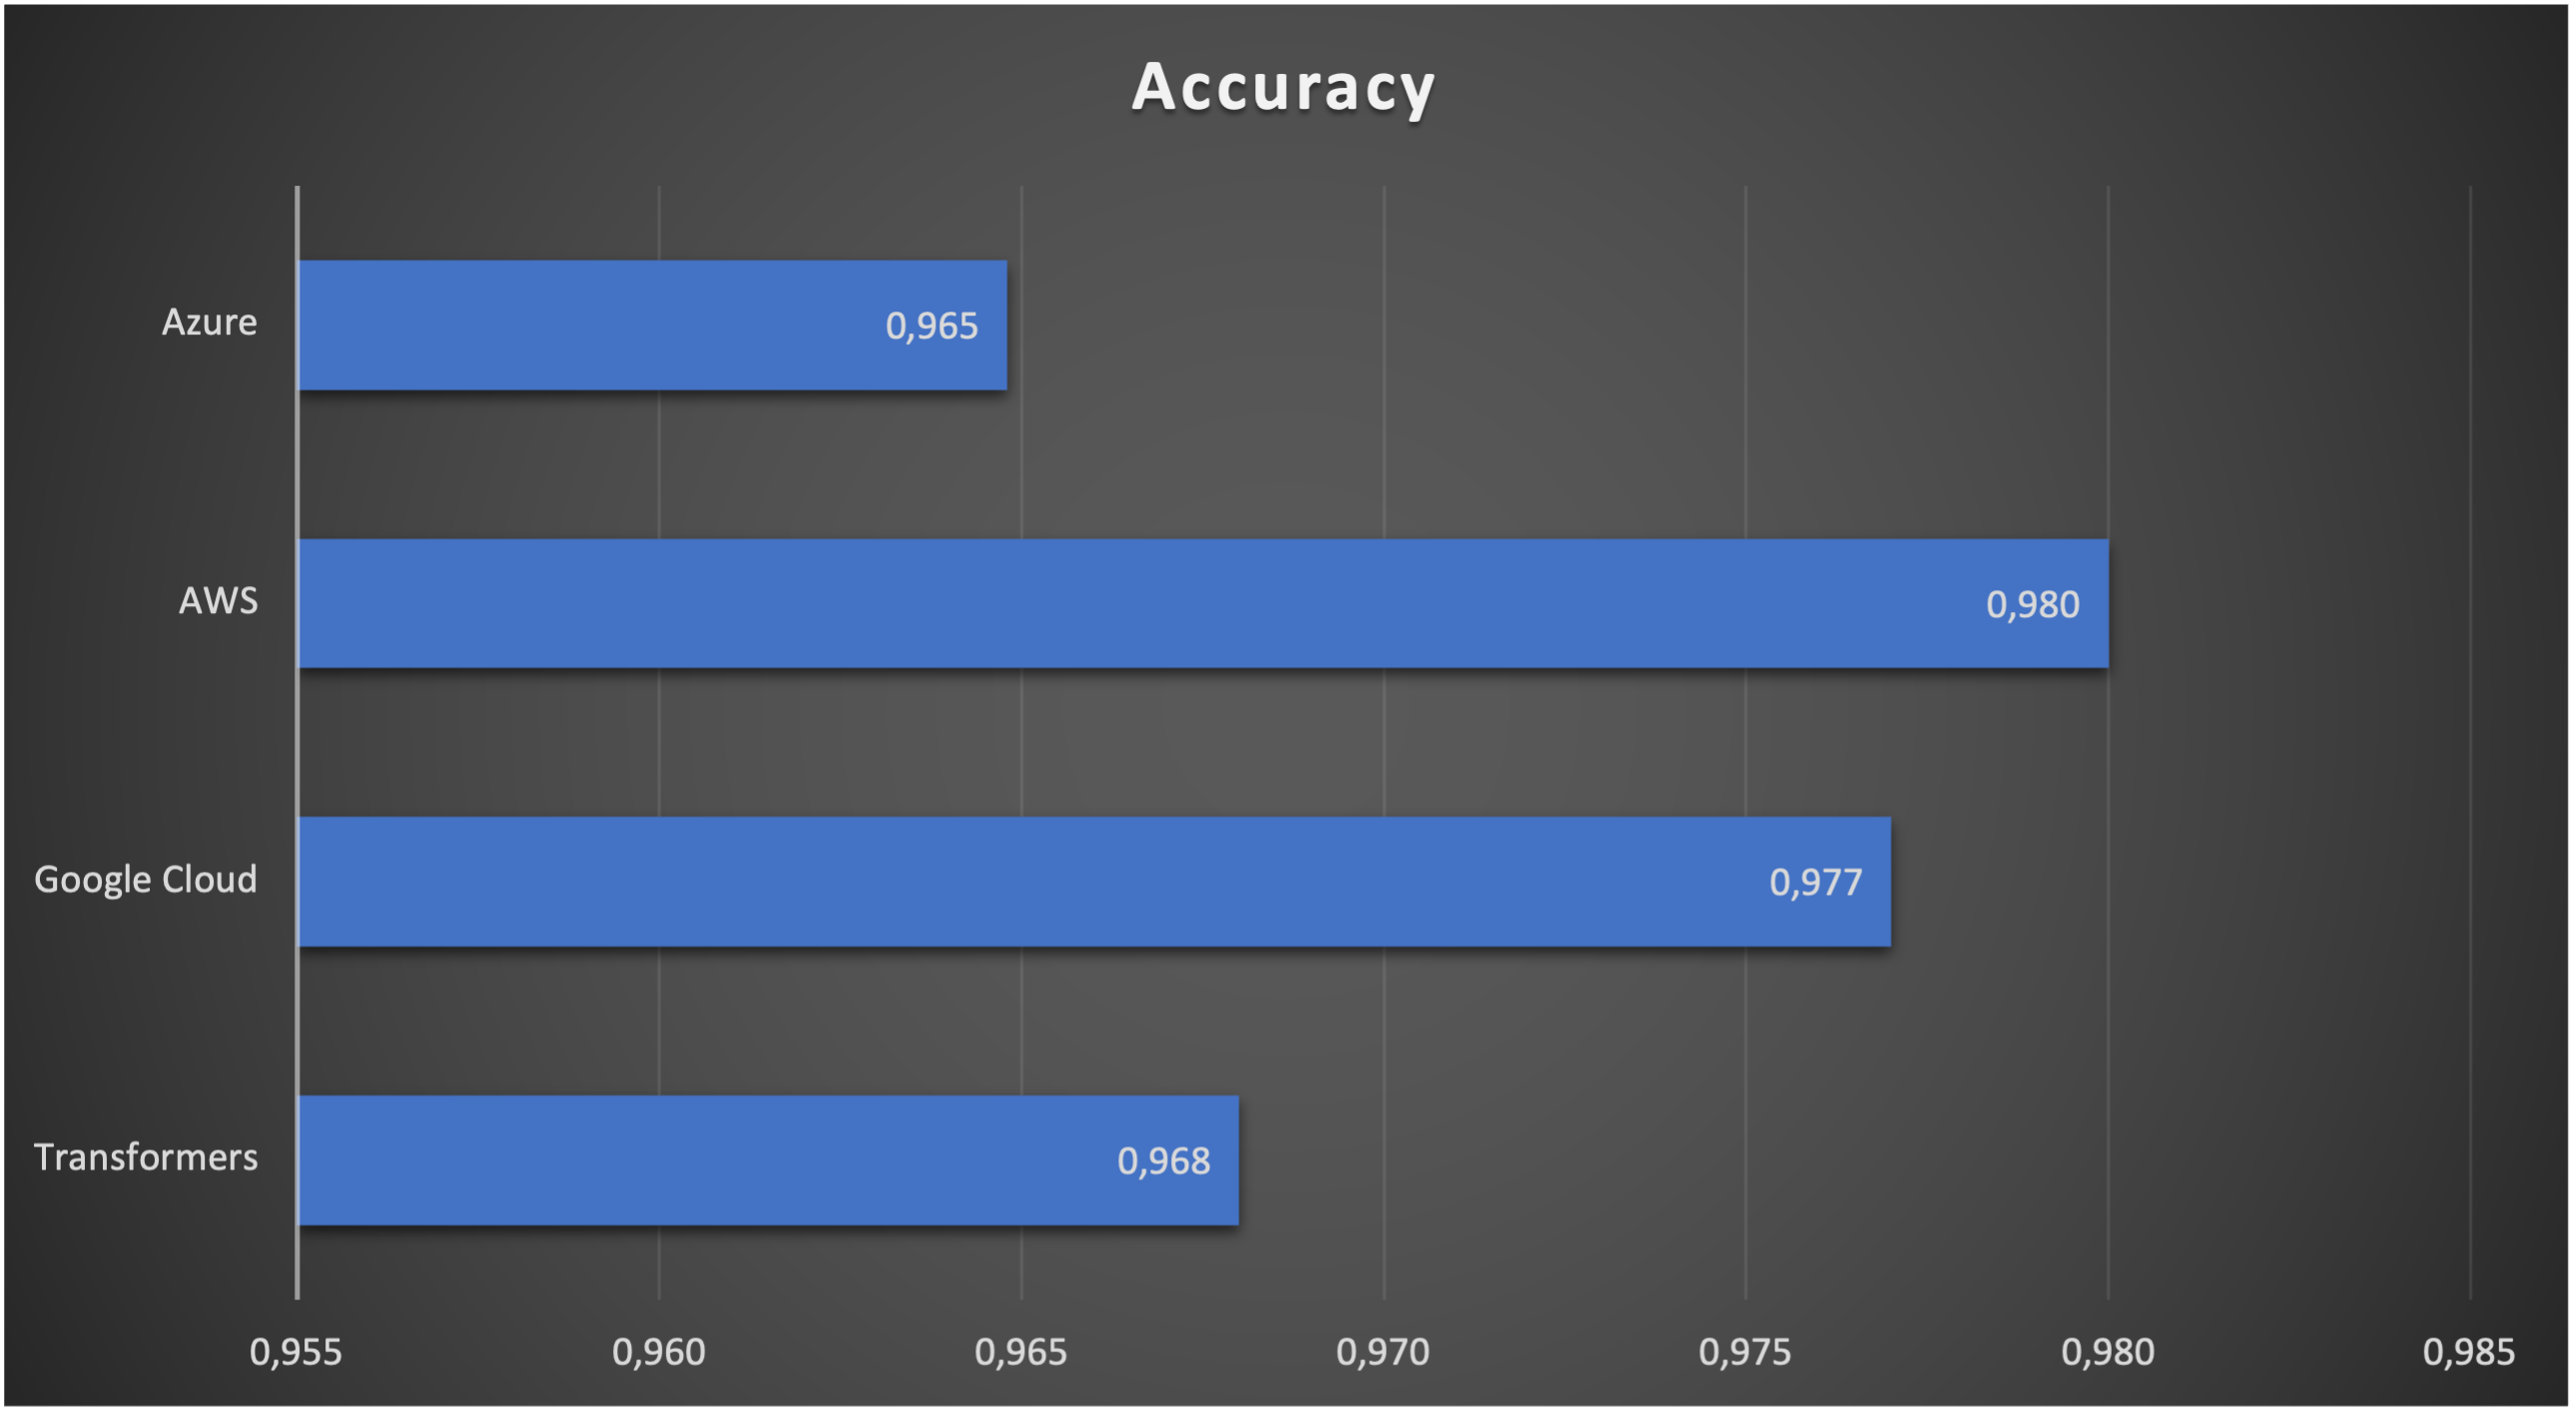
\includegraphics[width=10cm]{OBJECT.png}
\end{center}
\caption{ Zaznava objektov Accuracy rezultat}
\label{pic2}
\end{figure}


Pri zaznavi objektov je bil uporabljen  \hyperref[sec:coco]{\underline {COCO}} dataset.

Kot najboljša izbira za zaznavanje objektov pa se je izkazala storitev AWS SageMaker.


%----------------------------------------------------------------
% Poglavje (Chapter) 6
%----------------------------------------------------------------
\chapter{Zaključek}
\label{ch8}

Zaključimo lahko, da so trije največji ponudniki v oblaku po rezultatih zelo tesno skupaj, kakor pa lahko razberemo iz rezultatov pa je tudi odprtokodna rešitev zasedla prvo mesto.

 



% ---------------------------------------------------------------
% Appendix
% ---------------------------------------------------------------
%00\appendix
%\addcontentsline{toc}{chapter}{Razširjeni povzetek}
%\chapter{Title of the appendix 1}

%Example of the appendix.

%----------------------------------------------------------------
% SLO: bibliografija
% ENG: bibliography
%----------------------------------------------------------------
\bibliographystyle{elsarticle-num}

%----------------------------------------------------------------
% SLO: odkomentiraj za uporabo zunanje datoteke .bib (ne pozabi je potem prevesti!)
% ENG: uncomment to use .bib file (don't forget to compile it!)
%----------------------------------------------------------------
%\bibliography{bibliography}

%----------------------------------------------------------------
% SLO: zakomentiraj spodnji del, če uporabljaš zunanjo .bib datoteko
% ENG: comment the part below if using the .bib file
%----------------------------------------------------------------

\begin{thebibliography}{99}
\bibitem{hugging} Hugging Face. Dostopno na: \url{https://huggingface.co/learn/nlp-course/chapter1/4}  [Dostopano 10. 06. 2023].
\bibitem{transformers} Transformers. Dostopno na: \url{https://huggingface.co/learn/nlp-course/chapter2/1?fw=pt}  [Dostopano 10. 06. 2023].
\bibitem{google} Google Cloud. Dostopno na: \url{https://cloud.google.com/natural-language#section-1}  [Dostopano 10. 06. 2023].
\bibitem{vertex} Vertex AI. Dostopno na: \url{https://cloud.google.com/vertex-ai}  [Dostopano 10. 06. 2023].
\bibitem{aws} Amazon Web Services (AWS).  Dostopno na: \url{https://aws.amazon.com/}  [Dostopano 10. 06. 2023].
\bibitem{sage} Amazon SageMaker.  Dostopno na: \url{https://aws.amazon.com/sagemaker/}  [Dostopano 10. 06. 2023].
\bibitem{azure} Azure. Dostopno na: \url{https://azure.microsoft.com/en-us}  [Dostopano 10. 06. 2023].
\bibitem{cognitive} Azure Cognitive Services. Dostopno na: \url{https://azure.microsoft.com/en-gb/products/cognitive-services}  [Dostopano 10. 06. 2023].
\bibitem{ner} Named Entity Recognition. Dostopno na: \url{https://www.shaip.com/blog/named-entity-recognition-and-its-types/}  [Dostopano 10. 06. 2023].
\bibitem{sentiment} Sentiment Analysis. Dostopno na: \url{https://aws.amazon.com/what-is/sentiment-analysis/}  [Dostopano 10. 06. 2023].
\bibitem{povzetek} Summarization. Dostopno na: \url{https://huggingface.co/tasks/summarization}  [Dostopano 10. 06. 2023].
\bibitem{luscenje} Keyphrase Extraction. Dostopno na: \url{https://www.geeksforgeeks.org/keyphrase-extraction-in-nlp/}  [Dostopano 10. 06. 2023].
\bibitem{klasifikacija} Text Classification. Dostopno na: \url{https://huggingface.co/tasks/text-classification}  [Dostopano 10. 06. 2023].
\bibitem{object} Object Detection. Dostopno na: \url{https://huggingface.co/tasks/object-detection}  [Dostopano 10. 06. 2023].
\bibitem{truevsfalse} True vs. False and Positive vs. Negative. Dostopno na: \url{https://developers.google.com/machine-learning/crash-course/classification/true-false-positive-negative}  [Dostopano10. 06. 2023].
\bibitem{conll}Erik F. Tjong Kim Sang and Fien De Meulder  ``Introduction to the CoNLL-2003''. Dostopno na: \url{https://aclanthology.org/W03-0419.pdf}  [Dostopano
10. 06. 2023].
\bibitem{imdb} IMDB Dataset Reviews. Dostopno na: \url{https://www.kaggle.com/datasets/lakshmi25npathi/imdb-dataset-of-50k-movie-reviews}  [Dostopano 10. 06. 2023].
\bibitem{coco} COCO 2017 Dataset. Dostopno na: \url{https://www.kaggle.com/datasets/awsaf49/coco-2017-dataset}  [Dostopano 10. 06. 2023].
\bibitem{cnn} CNN dailymail Dataset. Dostopno na: \url{https://huggingface.co/datasets/cnn_dailymail}  [Dostopano 10. 06. 2023].
\bibitem{semeval} SemEval-datasetst. Dostopno na: \url{https://www.kaggle.com/datasets/azzouza2018/semevaldatadets?resource=download}  [Dostopano 10. 06. 2023].
\bibitem{accuracy} Accuracy. Dostopno na: \url{https://developers.google.com/machine-learning/crash-course/classification/accuracy}  [Dostopano
10. 06. 2023].
\bibitem{percision} Precision and Recall. Dostopno na: \url{https://developers.google.com/machine-learning/crash-course/classification/precision-and-recall}  [Dostopano
10. 06. 2023].
\end{thebibliography}

\end{document}
